\chapter{区间估计、假设检验与预测}
\label{chap:intervals-tests-prediction}

一台灌装机的标称灌装量是$500$ mL。质检员随机抽取$10$瓶，测得平均灌装量$501.5$ mL。第~\ref{chap:sample-estimation}章告诉我们怎样由样本得到这个点估计，第~\ref{chap:sampling-errors}章告诉我们样本均值在重复抽样中会波动多少。但实际工作提出的往往是另外三类问题：真正的平均灌装量大致在什么范围内？“平均灌装量就是$500$ mL”这个说法与数据是否相容？下一瓶会装多少？

这三个问题分别对应本章的三项统计任务：用区间圈定未知参数，用检验判断关于参数的陈述，用区间预测尚未观测的结果。它们使用的原料相同，都是统计量的抽样分布或参数的后验分布；差别在于所要覆盖或判断的对象不同，因而概率的含义也不同。第~\ref{sec:pred-intervals}节先构造均值、比例和方差的区间，并把后验可信区间与之比较；第~\ref{sec:pred-tests}节建立检验的共同概念，再按参数逐一构造检验，最后说明检验与区间如何互相转化；第~\ref{sec:pred-prediction}节把对象换成未来观测，说明预测区间为什么总比均值区间宽；第~\ref{sec:pred-regression}节在简单线性回归中把估计、区间、检验与预测放进同一个模型。

全章反复使用一组教学数据，便于比较不同方法对同一问题给出的回答。

\begin{example}[灌装量数据]
\label{ex:pred-filling-data}
从灌装机A随机抽取$10$瓶，灌装量（单位：mL，教学数据）为
\[
 501.8,\ 499.6,\ 502.4,\ 500.9,\ 503.1,\ 501.2,\ 499.9,\ 502.6,\ 501.5,\ 502.0.
\]
样本均值$\bar x=5015/10=501.5$。各观测与均值之差的平方和为$\sum_i(x_i-\bar x)^2=11.54$，于是修正样本方差$s^2=11.54/9\approx1.2822$，样本标准差$s\approx1.1324$，均值的估计标准误$s/\sqrt{10}\approx0.3581$。本章把这批数据看作正态总体$\mathcal N(\mu,\sigma^2)$的独立样本，除非另有说明。
\end{example}

本章沿用前几章的记号：$\Phi$是标准正态分布函数，$z_p=\Phi^{-1}(p)$是其下侧$p$分位数；$t_{k,p}$、$\chi^2_{k,p}$、$F_{k_1,k_2,p}$分别是自由度为$k$的$t$分布、卡方分布以及自由度为$(k_1,k_2)$的$F$分布的下侧$p$分位数。样本$X_1,\dots,X_n$的样本均值记$\bar X_n$，修正样本方差记$S_n^2$；不致混淆时省略下标$n$。参数为$\theta$时计算的概率与期望记作$\mathbb P_\theta$与$\mathbb E_\theta$。

\section{区间估计}
\label{sec:pred-intervals}

点估计$\bar x=501.5$没有告诉我们它离真值可能有多远。第~\ref{sec:samp-standard-error}节用标准误描述了估计量的典型波动幅度；本节更进一步，把这种波动换算成一个区间，并要求这个区间在重复抽样中以指定的概率覆盖真参数。我们先说明覆盖概率的含义和一般构造方法，再依次处理均值、比例与方差，最后把这些区间与由后验分布得到的区间相比较。

\subsection{置信区间与覆盖率}

\paragraph{区间端点是统计量}

设想质检员每天都抽$10$瓶、每天都报一个区间。今天的区间是由今天的样本算出来的，明天换一批样本，区间也随之改变。因此在抽样之前，区间的两个端点是样本的函数，即两个统计量；而要估计的平均灌装量$\mu$是一个固定但未知的数。说一个区间“可靠”，只能是说这种构造规则在反复使用时多半能把$\mu$圈住。

\begin{definition}[置信区间]
\label{def:pred-confidence-interval}
设样本$\bm X=(X_1,\dots,X_n)$的分布由参数$\theta\in\Theta$决定，$L(\bm X)\leq U(\bm X)$是两个统计量，$0<\alpha<1$。函数
\[
 C(\theta)=\mathbb P_\theta\bigl(L(\bm X)\leq\theta\leq U(\bm X)\bigr),\qquad\theta\in\Theta,
\]
称为随机区间$[L(\bm X),U(\bm X)]$的\term{覆盖概率}（coverage probability）。若对每个$\theta\in\Theta$都有$C(\theta)\geq1-\alpha$，则称$[L(\bm X),U(\bm X)]$为$\theta$的置信水平为$1-\alpha$的\term{置信区间}（confidence interval），$1-\alpha$称为\term{置信水平}（confidence level）。
\end{definition}

定义里的概率是对样本$\bm X$计算的，$\theta$在概率符号中只作为分布的标号出现。要求“对每个$\theta$”成立，是因为我们不知道真参数是哪一个，只能要求构造规则无论面对哪个参数都可靠。只允许取一侧的区间，例如$(-\infty,U(\bm X)]$，同样可以按此定义，称为单侧置信区间或置信上界。

一旦代入观测值，例如例~\ref{ex:pred-filling-t-interval}将由灌装量数据算得区间$[500.69,502.31]$，它就是两个确定的数。这时$\mu$要么在其中，要么不在，“$\mu$以$95\%$的概率落在$[500.69,502.31]$中”不是置信区间所能支持的说法；$95\%$描述的是产生这个区间的规则。图~\ref{fig:pred-coverage-simulation}把这种规则重复执行了$50$次：每次从同一个正态总体抽$10$个观测并按下文的$t$区间公式计算，大多数区间穿过真值所在的虚线，少数区间整个落在虚线一侧。

\begin{figure}[htbp]
  \centering
  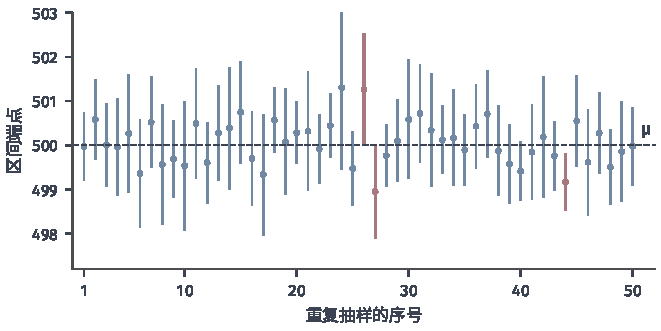
\includegraphics[width=112mm]{figures/01-basic-mathematics/05-probability-and-statistics-basics/matplotlib/pred-coverage-simulation/figure.pdf}
  \caption{同一构造规则的$50$次重复。每次从$\mathcal N(500,1.5^2)$独立抽取$10$个观测，计算$95\%$的$t$区间（竖线）与样本均值（圆点）；虚线是真均值$\mu=500$。红色的$3$个区间未覆盖真值，其余$47$个覆盖。区间的中心与长度都随样本变化，真值固定不动。模拟使用固定随机种子$20261028$。}
  \label{fig:pred-coverage-simulation}
\end{figure}

\paragraph{从标准化量反解参数}

怎样得到覆盖概率可控的区间？关键是找一个同时含样本与参数、而分布与参数无关的量。最简单的例子来自第~\ref{sec:samp-normal}节：正态样本且$\sigma$已知时，
\[
 Z=\frac{\bar X-\mu}{\sigma/\sqrt n}\sim\mathcal N(0,1),
\]
无论$\mu$取什么值，$Z$都服从标准正态分布。

\begin{definition}[枢轴量]
\label{def:pred-pivot}
若$Q(\bm X,\theta)$的分布在每个$\mathbb P_\theta$下都相同、不依赖$\theta$，则称$Q$为\term{枢轴量}（pivotal quantity）。
\end{definition}

有了枢轴量，构造分两步。第一步取其分布的两个分位数$q_{\alpha/2}$与$q_{1-\alpha/2}$，使$\mathbb P_\theta(q_{\alpha/2}\leq Q\leq q_{1-\alpha/2})=1-\alpha$对一切$\theta$成立；第二步把不等式$q_{\alpha/2}\leq Q(\bm X,\theta)\leq q_{1-\alpha/2}$对$\theta$解出来。若解集是一个区间$[L(\bm X),U(\bm X)]$，则两个事件相同，覆盖概率恰为$1-\alpha$。以$Z$为例，
\[
 -z_{1-\alpha/2}\leq\frac{\bar X-\mu}{\sigma/\sqrt n}\leq z_{1-\alpha/2}
 \iff
 \bar X-z_{1-\alpha/2}\frac{\sigma}{\sqrt n}\leq\mu\leq\bar X+z_{1-\alpha/2}\frac{\sigma}{\sqrt n},
\]
其中用到标准正态分布关于零对称，$z_{\alpha/2}=-z_{1-\alpha/2}$。本节后面的均值、方差区间都按这条路线构造，差别只在于枢轴量不同。

\paragraph{名义覆盖率、实际覆盖率与区间长度}

构造时要求的$1-\alpha$称为\term{名义覆盖率}（nominal coverage），覆盖概率$C(\theta)$的实际数值称为实际覆盖率。若枢轴量的分布准确已知，二者相等；若只用了近似分布，或样本取值离散，实际覆盖率可能低于或高于名义值，并且可能随$\theta$变化。评价一个区间方法，首先看实际覆盖率是否至少接近名义值。

覆盖率并不是唯一标准。区间$(-\infty,\infty)$的覆盖率永远是$1$，却没有提供任何信息。所以在覆盖率达到要求的方法中，我们希望区间尽量短。对同一个枢轴量，提高置信水平会换用更外侧的分位数，区间随之变长；增加样本量则通过$1/\sqrt n$缩短区间。下文比较不同方法时，总是同时看覆盖率与长度这两项。

\subsection{均值的置信区间}

均值区间按总体的已知程度分三种情形：正态且方差已知、正态而方差未知、只知道方差有限。前两种有精确的枢轴量，第三种只能依靠大样本近似。

\paragraph{正态总体、方差已知}

若$X_1,\dots,X_n$独立同分布于$\mathcal N(\mu,\sigma^2)$且$\sigma$已知，上一小节已经从$Z$得到
\begin{equation}
 \bar X\pm z_{1-\alpha/2}\frac{\sigma}{\sqrt n}.
 \label{eq:pred-z-interval}
\end{equation}
它的覆盖概率对每个$\mu$都恰好是$1-\alpha$，长度$2z_{1-\alpha/2}\sigma/\sqrt n$不随样本变化。

\begin{example}[方差已知时的灌装量区间]
\label{ex:pred-filling-z-interval}
假定设备手册给出灌装量的标准差$\sigma=1.5$ mL，并信任这一数值。对例~\ref{ex:pred-filling-data}，$95\%$置信区间为
\[
 501.5\pm1.96\times\frac{1.5}{\sqrt{10}}=501.5\pm0.930=[500.57,\,502.43].
\]
\end{example}

\paragraph{正态总体、方差未知：$t$区间}

实际中$\sigma$通常未知，自然的做法是用$S$代替它。代替后的量不再服从标准正态分布：分母也随样本波动，尾部会更厚。第~\ref{sec:samp-normal}节证明了，正态样本的$\bar X$与$S^2$相互独立，且$(n-1)S^2/\sigma^2\sim\chi^2_{n-1}$；第~\ref{sec:samp-t}节由此得到
\begin{equation}
 T=\frac{\bar X-\mu}{S/\sqrt n}\sim t_{n-1}.
 \label{eq:pred-t-pivot}
\end{equation}
$T$的分布不含$\mu$与$\sigma$，是枢轴量。$t$分布关于零对称，按同样的反解得到\term{$t$区间}（$t$ interval）
\begin{equation}
 \bar X\pm t_{n-1,1-\alpha/2}\frac{S}{\sqrt n}.
 \label{eq:pred-t-interval}
\end{equation}
对正态总体，它的覆盖概率对一切$(\mu,\sigma^2)$恰为$1-\alpha$。

$t$分位数总大于对应的正态分位数，这是为$\sigma$的估计误差付出的代价：$t_{2,0.975}\approx4.303$，$t_{4,0.975}\approx2.776$，$t_{9,0.975}\approx2.262$，$t_{29,0.975}\approx2.045$，$t_{99,0.975}\approx1.984$，随自由度增大逐渐接近$z_{0.975}\approx1.960$。小样本时差别显著，样本数十以上时差别已不大。

\begin{example}[方差未知时的灌装量区间]
\label{ex:pred-filling-t-interval}
不再假定$\sigma$已知。对例~\ref{ex:pred-filling-data}，$t_{9,0.975}\approx2.262$，估计标准误$s/\sqrt{10}\approx0.3581$，故$95\%$的$t$区间为
\[
 501.5\pm2.262\times0.3581=501.5\pm0.810=[500.69,\,502.31].
\]
这个区间反而比例~\ref{ex:pred-filling-z-interval}窄，原因是这批样本的$s\approx1.13$恰好小于手册给出的$\sigma=1.5$。在重复抽样的平均意义下，$t$区间比已知$\sigma$时的区间长；对一个具体样本，二者谁长取决于$s$的大小。
\end{example}

\paragraph{一般总体的大样本区间}

总体不是正态时，$T$不再精确服从$t_{n-1}$。若$X_1,\dots,X_n$独立同分布，方差$\sigma^2$有限且大于零，第~\ref{sec:samp-clt}节的中心极限定理说明$\sqrt n(\bar X_n-\mu)/\sigma$的分布函数逐点收敛于$\Phi$；第~\ref{sec:samp-consistency}节又说明$S_n$依概率收敛于$\sigma$。把分母中的$\sigma$换成$S_n$相当于乘上一个依概率趋于$1$的因子$\sigma/S_n$，第~\ref{sec:samp-clt}节用Slutsky定理说明了这种替换不改变极限分布。于是对每个固定的总体分布，
\[
 \lim_{n\to\infty}\mathbb P\Bigl(\Bigl|\frac{\bar X_n-\mu}{S_n/\sqrt n}\Bigr|\leq z_{1-\alpha/2}\Bigr)=1-\alpha,
\]
区间$\bar X_n\pm z_{1-\alpha/2}S_n/\sqrt n$的覆盖概率趋于名义值。实际中常用$t$分位数代替$z_{1-\alpha/2}$，两者在大样本下几乎相同，而$t$分位数在小样本时略为保守。

这个结论是渐近性质：它说的是$n\to\infty$时的极限，并不保证某个固定的$n$已经足够，也不保证收敛对所有总体同样快。总体越偏斜，需要的样本量越大。

\begin{example}[偏斜总体下的$t$区间]
\label{ex:pred-exponential-coverage}
设总体是均值为$1$的指数分布。用固定随机种子$20261028$各重复$200000$次，名义$95\%$的$t$区间的实际覆盖率约为：$n=5$时$0.88$，$n=10$时$0.90$，$n=30$时$0.93$，$n=100$时$0.94$。覆盖率随$n$增大而逼近$0.95$，但小样本时明显不足。未覆盖的情形也不对称：$n=10$时约$9.6\%$的区间整个落在真均值左侧，只有约$0.4\%$落在右侧。指数分布右偏：样本中没有出现大观测时，样本均值偏低，样本标准差也偏小，区间又低又短，于是整个落在真均值左侧；出现大观测时样本均值偏高，但样本标准差同时变大，区间很宽，往往仍能覆盖真值。
\end{example}

\subsection{比例的置信区间}

\paragraph{正态近似区间}

灌装线上的另一项指标是封口不合格率$p$。把第$i$瓶不合格记为$X_i=1$、合格记为$X_i=0$，则$X_i\sim\operatorname{Bernoulli}(p)$，不合格数$S=\sum_iX_i\sim\operatorname{Bin}(n,p)$，样本比例$\hat p=S/n$就是样本均值。于是比例的区间是均值区间的特例：Bernoulli总体的方差为$p(1-p)$，用$\hat p(1-\hat p)$估计它，大样本区间成为
\begin{equation}
 \hat p\pm z_{1-\alpha/2}\sqrt{\frac{\hat p(1-\hat p)}{n}}.
 \label{eq:pred-wald-interval}
\end{equation}
这个区间称为\term{Wald区间}（Wald interval）。它只依赖中心极限定理，因此只是近似区间。

\begin{example}[封口不合格率的Wald区间]
\label{ex:pred-wald}
抽查$n=40$瓶，发现$s=6$瓶封口不合格，$\hat p=0.15$。估计标准误$\sqrt{0.15\times0.85/40}\approx0.0565$，$95\%$的Wald区间为$0.15\pm1.96\times0.0565=[0.039,\,0.261]$。

再看一个极端情形：抽查$n=20$瓶，全部合格，$s=0$。这时$\hat p=0$，估计标准误也是$0$，式~\eqref{eq:pred-wald-interval}给出单点区间$[0,0]$，等于断言不合格率恰好为零。这显然过于自信。
\end{example}

例中的退化并非偶然。Wald区间有两处近似：用正态分布近似离散的二项分布，以及用$\hat p$代替标准误中的$p$。当$n$不大或$p$接近$0$、$1$时，二项分布明显偏斜，两处近似都不可靠。图~\ref{fig:pred-proportion-coverage}按二项概率精确计算了$n=30$时Wald区间的覆盖概率：在中间区域它多数时候低于$0.95$，并随$p$锯齿状跳动；靠近边界时覆盖率急剧下降，$p=0.05$处约为$0.78$。

\begin{figure}[htbp]
  \centering
  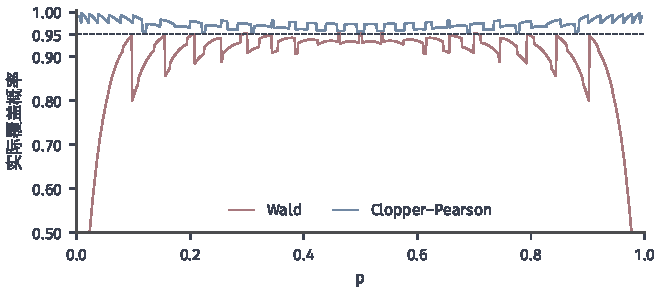
\includegraphics[width=112mm]{figures/01-basic-mathematics/05-probability-and-statistics-basics/matplotlib/pred-proportion-coverage/figure.pdf}
  \caption{$n=30$时两种名义$95\%$比例区间的实际覆盖概率，按$C(p)=\sum_{s}\mathbb P_p(S=s)\,\mathbb I_{\{p\in[L(s),U(s)]\}}$精确计算。红线为Wald区间，在大部分$p$处低于虚线$0.95$，靠近$0$与$1$时急剧下降；蓝线为Clopper--Pearson区间，处处不低于$0.95$，多数位置明显高于它。锯齿来自$S$只能取整数。}
  \label{fig:pred-proportion-coverage}
\end{figure}

图中的锯齿说明了离散分布的一个特点。$S$只取$0,1,\dots,n$这$n+1$个值，因此区间也只有$n+1$个可能的结果。$p$连续变化时，某个$s$对应的区间端点一旦越过$p$，这个$s$的概率就整块进入或离开覆盖概率，覆盖率随之跳动。

\paragraph{由二项尾概率反求：精确区间}

既然问题出在近似，我们改为直接使用二项分布。思路是：观测到$s$之后，把那些“使观测值落在过远尾部”的$p$排除掉。若$p$很小，出现$s$或更多不合格的概率$\mathbb P_p(S\geq s)$就很小；若$p$很大，出现$s$或更少的概率$\mathbb P_p(S\leq s)$很小。两侧各留$\alpha/2$，即得下面的区间。

\begin{definition}[Clopper--Pearson区间]
\label{def:pred-clopper-pearson}
设$S\sim\operatorname{Bin}(n,p)$，观测值为$s$。当$s\geq1$时，令$p_L(s)$为方程$\mathbb P_p(S\geq s)=\alpha/2$关于$p$的解；当$s=0$时，令$p_L(0)=0$。当$s\leq n-1$时，令$p_U(s)$为方程$\mathbb P_p(S\leq s)=\alpha/2$关于$p$的解；当$s=n$时，令$p_U(n)=1$。区间$[p_L(S),p_U(S)]$称为\term{Clopper--Pearson区间}（Clopper--Pearson interval），也称精确区间。
\end{definition}

定义中的方程有唯一解，依据是二项尾概率关于$p$的单调性：对固定的$s\geq1$，$\mathbb P_p(S\geq s)$随$p$严格增加，从$p=0$时的$0$连续增到$p=1$时的$1$。直观上，成功概率越大，成功次数越容易达到$s$。严格的说明可以用一个耦合构造：取$U_1,\dots,U_n$独立同分布于$\operatorname U(0,1)$，令$S_p=\sum_i\mathbb I_{\{U_i\leq p\}}$，则$S_p\sim\operatorname{Bin}(n,p)$；当$p<p'$时每一项$\mathbb I_{\{U_i\leq p\}}\leq\mathbb I_{\{U_i\leq p'\}}$，故$S_p\leq S_{p'}$，从而$\mathbb P(S_p\geq s)\leq\mathbb P(S_{p'}\geq s)$。这说明了单调不减。至于严格增加与连续性，$\mathbb P_p(S\geq s)=\sum_{k\geq s}\binom nk p^k(1-p)^{n-k}$是$p$的多项式，逐项求导后相邻项相消，只剩$n\binom{n-1}{s-1}p^{s-1}(1-p)^{n-s}$，它在$0<p<1$上为正。同理，$\mathbb P_p(S\leq s)$随$p$严格减少。

\begin{theorem}[Clopper--Pearson区间的覆盖]
\label{thm:pred-clopper-pearson-coverage}
对每个$p\in[0,1]$，都有
\[
 \mathbb P_p\bigl(p_L(S)\leq p\leq p_U(S)\bigr)\geq1-\alpha.
\]
\end{theorem}

\begin{proof}
固定真参数$p$，只需证明区间漏掉$p$的两种情形各自的概率小于$\alpha/2$。对整数$s$，记尾概率$g(s)=\mathbb P_p(S\geq s)$，这里$p$是固定的真参数。先看$p<p_L(s)$在哪些$s$上发生。$s=0$时$p_L=0$，不会发生；$s\geq1$时，$p_L(s)$是方程$\mathbb P_{p'}(S\geq s)=\alpha/2$关于$p'$的解，而左边随$p'$严格增加，所以$p<p_L(s)$当且仅当$g(s)<\alpha/2$。又$g(s)$随$s$递减，满足$g(s)<\alpha/2$的$s$构成一个右端集合$\{s:s\geq s^*\}$，其中$s^*$是使$g(s)<\alpha/2$的最小整数（若不存在，此情形概率为$0$）。于是
\[
 \mathbb P_p\bigl(p<p_L(S)\bigr)=\mathbb P_p(S\geq s^*)=g(s^*)<\frac\alpha2.
\]
对$p>p_U(S)$作对称的论证，得到其概率也小于$\alpha/2$。两种情形互斥，漏掉$p$的概率小于$\alpha$。
\end{proof}

证明的最后一步只能得到“小于$\alpha/2$”而不是“等于”，正是离散性所致：$g(s^*)$是尾概率函数在整数点上的取值，一般不会恰好落在$\alpha/2$上。因此Clopper--Pearson区间是\emph{保守}的，实际覆盖率通常高于名义值。图~\ref{fig:pred-proportion-coverage}中的蓝线显示了这一点：覆盖率处处不低于$0.95$，多数位置在$0.96$以上，靠近边界时接近$1$。保守换来的代价是区间较长。

计算上，$p_L$与$p_U$可以用Beta分布的分位数表示：$p_L(s)$是$\operatorname{Beta}(s,n-s+1)$的$\alpha/2$分位数，$p_U(s)$是$\operatorname{Beta}(s+1,n-s)$的$1-\alpha/2$分位数。这来自恒等式$\mathbb P_p(S\geq s)=\mathbb P(B\leq p)$，其中$B\sim\operatorname{Beta}(s,n-s+1)$：上面求得的导数$n\binom{n-1}{s-1}p^{s-1}(1-p)^{n-s}$恰是$\operatorname{Beta}(s,n-s+1)$的密度，两边在$p=0$处又都为$0$。

\begin{example}[两种比例区间的比较]
\label{ex:pred-clopper-pearson}
对$n=40$、$s=6$，Clopper--Pearson区间约为$[0.057,\,0.298]$，比Wald区间$[0.039,\,0.261]$长约$0.02$，并且整体右移：二项分布在$p$较小时右偏，精确区间把这种不对称保留下来。

对$n=20$、$s=0$，$p_L=0$，$p_U$满足$(1-p)^{20}=0.025$，解得$p_U=1-0.025^{1/20}\approx0.168$。区间$[0,\,0.168]$承认，即使$20$瓶全部合格，不合格率仍可能高达约$17\%$；Wald区间的$[0,0]$则完全忽略了这种可能。
\end{example}

两种区间各有用途。Wald区间形式简单，在$n\hat p$与$n(1-\hat p)$都较大时表现尚可；Clopper--Pearson区间在任何$n$下都保证覆盖率，适合样本小或比例接近边界的情形。实践中还有一些覆盖率更接近名义值、长度更短的折中方法，这里不展开。

\subsection{方差的置信区间}

灌装量的波动大小同样关系质量：均值合格而方差过大，仍会有许多瓶偏离标称。我们需要总体方差$\sigma^2$的区间。

\paragraph{卡方枢轴量}

第~\ref{sec:samp-chi-square}节证明，若$X_1,\dots,X_n$独立同分布于$\mathcal N(\mu,\sigma^2)$，则
\[
 \frac{(n-1)S^2}{\sigma^2}\sim\chi^2_{n-1}.
\]
这个量的分布不含$\mu$与$\sigma^2$，是枢轴量。取卡方分布的两个分位数，
\[
 \chi^2_{n-1,\alpha/2}\leq\frac{(n-1)S^2}{\sigma^2}\leq\chi^2_{n-1,1-\alpha/2}
 \iff
 \frac{(n-1)S^2}{\chi^2_{n-1,1-\alpha/2}}\leq\sigma^2\leq\frac{(n-1)S^2}{\chi^2_{n-1,\alpha/2}},
\]
其中对正数取倒数时不等号方向反转。于是$\sigma^2$的置信水平为$1-\alpha$的区间为
\begin{equation}
 \Bigl[\frac{(n-1)S^2}{\chi^2_{n-1,1-\alpha/2}},\ \frac{(n-1)S^2}{\chi^2_{n-1,\alpha/2}}\Bigr].
 \label{eq:pred-variance-interval}
\end{equation}
对两端开平方，就得到$\sigma$的区间，覆盖概率不变，因为平方根是严格增函数。

\begin{example}[灌装量方差的区间]
\label{ex:pred-filling-variance-interval}
对例~\ref{ex:pred-filling-data}，$(n-1)s^2=11.54$，$\chi^2_{9,0.025}\approx2.700$，$\chi^2_{9,0.975}\approx19.023$。$\sigma^2$的$95\%$置信区间为
\[
 \Bigl[\frac{11.54}{19.023},\ \frac{11.54}{2.700}\Bigr]\approx[0.607,\,4.273],
\]
相应$\sigma$的区间约为$[0.779,\,2.067]$。点估计$s^2\approx1.282$距左端点$0.675$，距右端点$2.991$。
\end{example}

例中的区间明显不对称，原因在于卡方分布右偏：它的左尾短、右尾长，两个分位数到中心的距离不同；而反解时又取了倒数，把右尾的长度转移到了区间的右端。这种不对称也符合直观：$\sigma^2$只能取正值，样本方差的误差更接近按比例发生，而不是按差值发生。例如样本方差只有真方差的一半，与样本方差是真方差的两倍，都是小样本中常见的偏离，前者对应的真值在点估计右侧$s^2$处，后者对应的真值在左侧$s^2/2$处，所以区间向右伸得更远。只有$10$个观测时，方差的区间宽到上下端点相差七倍，说明小样本几乎无法精确确定波动大小。

\paragraph{对正态性的依赖}

均值的$t$区间在非正态总体下至少还有大样本的保障，方差的卡方区间却没有。原因可以通过比较$S^2$的波动来看。由于$S^2$与$\frac1n\sum_i(X_i-\mu)^2$只差一个在大样本下可以忽略的项，后者又是独立同分布变量$(X_i-\mu)^2$的样本均值，按中心极限定理，$\sqrt n(S^2-\sigma^2)$近似服从均值为$0$、方差为$\operatorname{Var}\bigl((X-\mu)^2\bigr)=\mu_4-\sigma^4$的正态分布，其中$\mu_4=\mathbb E(X-\mu)^4$为四阶中心矩（这里假设它有限）。

卡方区间的长度是按正态总体设计的。正态总体的$\mu_4=3\sigma^4$，故上式方差为$2\sigma^4$；这与卡方结论相符，因为由$\chi^2_{n-1}$的方差$2(n-1)$得$\operatorname{Var}(S^2)=2\sigma^4/(n-1)$，乘以$n$后趋于$2\sigma^4$。若总体的$\mu_4$大于$3\sigma^4$，即尾部比正态厚，$S^2$的真实波动就大于卡方区间所预设的波动，区间偏短；而且这种偏差不随$n$增大而消失，因为两者的比值$(\mu_4-\sigma^4)/(2\sigma^4)$与$n$无关。

\begin{example}[指数总体下的方差区间]
\label{ex:pred-variance-nonnormal}
均值为$1$的指数分布有$\sigma^2=1$，$\mu_4=9$，$S^2$的大样本方差是正态情形的$(9-1)/2=4$倍，标准差是$2$倍。按上面的近似，卡方区间实际只覆盖$|N|\leq1.96/2$的情形，$N$为标准正态，故$n$很大时实际覆盖率趋于$2\Phi(0.98)-1\approx0.673$。模拟（种子$20261028$，各重复$200000$次）给出的实际覆盖率为：$n=5$时$0.82$，$n=10$时$0.77$，$n=30$时$0.71$，$n=100$时$0.69$。样本越多，覆盖率反而越接近这个偏低的极限。
\end{example}

所以方差区间~\eqref{eq:pred-variance-interval}的精确性完全建立在正态假设之上，不能以“样本量足够大”为理由用于非正态总体。使用前应当检查数据是否有明显的偏斜或厚尾。

\subsection{后验可信区间}

前面几小节把参数视为固定未知的数。第~\ref{sec:est-bayes}节介绍了另一种做法：给参数指定先验分布，观测数据后得到后验分布，后验分布直接描述了在当前信息下参数各种取值的可能性。由后验分布同样可以给出参数范围。

\paragraph{等尾可信区间}

后验分布已经给出了参数落在任意范围内的概率，因此只需挑选一个后验概率达到要求的区间。

\begin{definition}[可信区间]
\label{def:pred-credible-interval}
给定观测数据$\bm x$与参数$\theta$的后验分布。若区间$[a,b]$满足$\mathbb P(a\leq\theta\leq b\mid\bm x)=1-\alpha$，则称它为$\theta$的后验概率为$1-\alpha$的\term{可信区间}（credible interval）。取$a$、$b$分别为后验分布的$\alpha/2$与$1-\alpha/2$分位数，得到\term{等尾可信区间}（equal-tailed credible interval）。
\end{definition}

满足要求的区间不止一个；等尾区间两侧各留$\alpha/2$的后验概率，计算最简单。后验分布不对称时，也可以选取长度最短的区间，这里不展开。我们用第~\ref{sec:est-posterior}节的两个共轭模型计算等尾区间。

\begin{example}[不合格率的可信区间]
\label{ex:pred-beta-credible}
在Beta--Bernoulli模型中，先验$p\sim\operatorname{Beta}(a,b)$，观测$n$次中有$s$次成功后，后验为$\operatorname{Beta}(a+s,\,b+n-s)$。取均匀先验$\operatorname{Beta}(1,1)$，对例~\ref{ex:pred-wald}的$n=40$、$s=6$，后验为$\operatorname{Beta}(7,35)$，其$0.025$与$0.975$分位数约为$0.072$与$0.292$。因此$[0.072,\,0.292]$是$p$的$95\%$等尾可信区间：在均匀先验和观测数据下，$p$落在其中的后验概率为$0.95$。它与Clopper--Pearson区间$[0.057,\,0.298]$接近，但含义不同，下面再作比较。
\end{example}

\begin{example}[灌装量均值的可信区间]
\label{ex:pred-normal-credible}
设灌装量$X_i\mid\mu\sim\mathcal N(\mu,\sigma^2)$相互独立，$\sigma^2=2.25$已知，先验$\mu\sim\mathcal N(\mu_0,\tau_0^2)$。第~\ref{sec:est-posterior}节得到后验仍为正态：后验精度是先验精度与数据精度之和，
\[
 \frac1{\tau_n^2}=\frac1{\tau_0^2}+\frac n{\sigma^2},
\]
后验均值$\mu_n$是先验均值与样本均值按各自精度加权的平均，
\[
 \mu_n=\tau_n^2\Bigl(\frac{\mu_0}{\tau_0^2}+\frac{n\bar x}{\sigma^2}\Bigr).
\]
取$\mu_0=500$、$\tau_0=1$（相信设备大致按标称灌装），对例~\ref{ex:pred-filling-data}的$n=10$、$\bar x=501.5$，后验精度为$1+10/2.25\approx5.444$，$\tau_n^2\approx0.1837$，$\tau_n\approx0.429$，后验均值
\[
 \mu_n\approx0.1837\times\Bigl(500+\frac{10\times501.5}{2.25}\Bigr)\approx501.22.
\]
$95\%$等尾可信区间为$501.22\pm1.96\times0.429=[500.38,\,502.06]$。与例~\ref{ex:pred-filling-z-interval}的置信区间$[500.57,\,502.43]$相比，它略窄，中心向先验均值$500$收缩了约$0.28$。
\end{example}

\paragraph{两种概率含义的比较}

可信区间和置信区间都写成“参数在某个范围内”，但其中的概率来自不同的随机性。置信区间的$1-\alpha$是对样本计算的：参数固定，区间随样本变化，规则在重复抽样中以概率$1-\alpha$覆盖参数。可信区间的$1-\alpha$是对参数计算的：数据固定，参数按后验分布变化，它落在区间中的后验概率为$1-\alpha$。所以对一次观测得到的可信区间，可以说“在给定先验与模型下，$\mu$在$[500.38,502.06]$中的概率是$0.95$”；对置信区间则不能这样说。

反过来，可信区间也不自动具有置信区间的保证。把例~\ref{ex:pred-normal-credible}的构造规则当作一个频率方法来检验：真均值固定为$\mu$，反复抽样并每次计算可信区间，覆盖概率是多少？后验均值$\mu_n=w\mu_0+(1-w)\bar X$，其中$w=\tau_n^2/\tau_0^2\approx0.184$，因此$\mu_n-\mu=w(\mu_0-\mu)+(1-w)(\bar X-\mu)$服从均值为$w(\mu_0-\mu)$、标准差为$(1-w)\sigma/\sqrt n\approx0.387$的正态分布，其中均值就是偏差。覆盖概率是这个正态变量落在$[-1.96\tau_n,\,1.96\tau_n]=[-0.840,\,0.840]$中的概率，计算得真均值为$500$时覆盖率约$0.97$，为$501.5$时约$0.93$，为$503$时只有约$0.77$。先验越偏离真值，频率覆盖率越低。先验恰当时，可信区间提供了置信区间所不能给出的直接概率陈述；先验不恰当时，它的频率性质可能很差。样本量增大时，数据精度$n/\sigma^2$压倒先验精度，$w\to0$，两种区间趋于一致。

\section{假设检验}
\label{sec:pred-tests}

区间回答“参数大概在哪里”，而许多实际问题要求对一个具体陈述作出判断：灌装机的平均灌装量是不是标称的$500$ mL？新测量方法与旧方法是否有系统差异？不合格率是否超过了合同规定的$5\%$？\term{假设检验}（hypothesis testing）把这类陈述写成关于参数的假设，并规定在数据达到什么程度时否定它。

本节前三个小节建立所有检验共有的概念：如何表述假设与拒绝域，判断可能犯哪两类错误，以及怎样用$p$值报告证据的强弱。接着按待检验的参数，依次处理单总体均值、两总体均值、比例与方差。最后一个小节说明检验与置信区间其实是同一组构造的两种读法。

\subsection{原假设、备择假设与拒绝域}

\paragraph{把陈述写成参数集合}

对一个统计模型，参数集$\Theta$中的每个值描述一种可能的总体。关于总体的陈述，例如“平均灌装量等于$500$”，就对应$\Theta$的一个子集。检验总是在两个互不相交的子集之间作选择。

\begin{definition}[原假设与备择假设]
\label{def:pred-hypotheses}
设参数集$\Theta$被分成两个不相交的非空子集$\Theta_0$与$\Theta_1$。陈述$H_0:\theta\in\Theta_0$称为\term{原假设}（null hypothesis），$H_1:\theta\in\Theta_1$称为\term{备择假设}（alternative hypothesis）。若$\Theta_0$只含一个点，称$H_0$为简单假设，否则称为复合假设。
\end{definition}

两个假设的地位并不对称。检验的逻辑是：先假定$H_0$成立，再看数据是否与之明显矛盾；只有矛盾足够明显，才否定$H_0$，转而采纳$H_1$。因此$H_0$通常是“没有差异”“符合标准”这类默认陈述，而希望用数据证明的结论放在$H_1$中。

以灌装量均值$\mu$为例，按所关心的问题可以写出三种检验问题：
\begin{itemize}
  \item 只关心是否偏离标称：$H_0:\mu=500$，$H_1:\mu\neq500$，称为\term{双侧检验}（two-sided test）；
  \item 厂方关心是否多装造成浪费：$H_0:\mu\leq500$，$H_1:\mu>500$；
  \item 消费者关心是否少装：$H_0:\mu\geq500$，$H_1:\mu<500$。
\end{itemize}
后两种只关心一个方向，称为\term{单侧检验}（one-sided test）。同一批数据面对不同的问题，可能得出不同的结论，所以检验问题必须在看数据之前根据实际需要确定。

\paragraph{拒绝域的构造}

写出假设之后，还要事先规定：数据呈现什么样子时否定$H_0$。这个规定由一个统计量和它的一组取值组成。

\begin{definition}[检验统计量与拒绝域]
\label{def:pred-rejection-region}
一个检验（test）由统计量$T(\bm X)$与集合$R$组成：观测到$T(\bm x)\in R$时拒绝$H_0$，否则不拒绝$H_0$。$T$称为\term{检验统计量}（test statistic），$R$称为\term{拒绝域}（rejection region）。
\end{definition}

拒绝域应当由“在$H_0$下不太可能、而在$H_1$下相对更可能”的取值组成。前一半要求$R$在$H_0$下的概率小，这需要知道$T$在$H_0$下的抽样分布；后一半决定$R$放在哪一侧：$H_1:\mu>500$时，样本均值偏大才是不利于$H_0$的证据，$R$应放在右尾；双侧问题中两个方向的偏离都算，$R$分在两尾。

\begin{example}[灌装量均值的双侧检验]
\label{ex:pred-filling-two-sided}
对例~\ref{ex:pred-filling-data}检验$H_0:\mu=500$，$H_1:\mu\neq500$，取
\[
 T=\frac{\bar X-500}{S/\sqrt{10}}.
\]
$H_0$成立时，由式~\eqref{eq:pred-t-pivot}，$T\sim t_9$。取拒绝域$R=\{|t|>t_{9,0.975}\}=\{|t|>2.262\}$，则$H_0$下拒绝的概率恰为$0.05$。观测值
\[
 t=\frac{501.5-500}{0.3581}\approx4.19>2.262,
\]
落入拒绝域，拒绝$H_0$：数据表明平均灌装量偏离了$500$ mL。
\end{example}

若把问题换成消费者关心的$H_0:\mu\geq500$对$H_1:\mu<500$，拒绝域应为左尾$\{t<-t_{9,0.95}\}=\{t<-1.833\}$。观测值$t\approx4.19$是正数，远离拒绝域，不拒绝$H_0$：数据没有显示少装。统计量相同，问题不同，结论也不同。

\subsection{两类错误与检验功效}

\paragraph{两类错误}

检验根据随机样本作出判断，判断就可能出错。真参数在$\Theta_0$或$\Theta_1$中，检验结果是拒绝或不拒绝，两两组合出四种情形，其中两种是错误：
\begin{center}
\begin{tabular}{lll}
  \toprule
  & 不拒绝$H_0$ & 拒绝$H_0$\\
  \midrule
  $H_0$为真 & 正确 & \term{第一类错误}（type I error）\\
  $H_1$为真 & \term{第二类错误}（type II error） & 正确\\
  \bottomrule
\end{tabular}
\end{center}
两类错误的概率都可以由一个函数统一表示。

\begin{definition}[功效函数与显著性水平]
\label{def:pred-power}
检验的\term{功效函数}（power function）是$\theta\mapsto\gamma(\theta)=\mathbb P_\theta\bigl(T(\bm X)\in R\bigr)$，即参数为$\theta$时拒绝$H_0$的概率。若
\[
 \sup_{\theta\in\Theta_0}\gamma(\theta)\leq\alpha,
\]
称检验的\term{显著性水平}（significance level）为$\alpha$。对$\theta\in\Theta_1$，$\gamma(\theta)$称为检验在$\theta$处的\term{功效}（power），$1-\gamma(\theta)$是在该处犯第二类错误的概率。
\end{definition}

显著性水平控制第一类错误：无论$H_0$中的哪个参数为真，错误拒绝的概率都不超过$\alpha$。第二类错误则没有统一的上界：备择参数离$\Theta_0$越近，越难与$H_0$区分，功效可以低到接近$\alpha$。所以谈论功效时必须指明是在哪个备择参数处。

两类错误此消彼长。图~\ref{fig:pred-error-types}画出单侧检验统计量在$H_0$与某个备择下的两条抽样分布。临界值右移，$\alpha$区域缩小，而$\beta$区域扩大。常规做法是先把$\alpha$固定在较小的值上，例如$0.05$，再在此约束下尽量提高功效。这正对应了两个假设的不对称：错误地否定默认陈述被视为更严重的错误。

\begin{figure}[htbp]
  \centering
  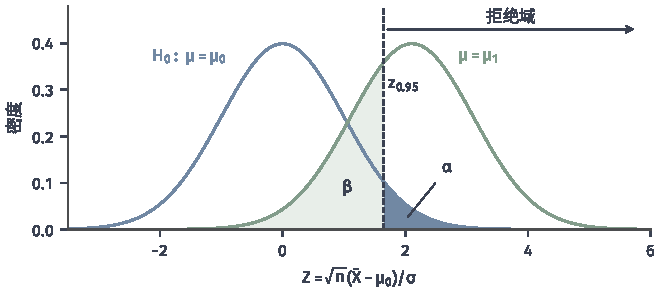
\includegraphics[width=112mm]{figures/01-basic-mathematics/05-probability-and-statistics-basics/matplotlib/pred-error-types/figure.pdf}
  \caption{单侧$z$检验的两类错误。蓝线是$H_0:\mu=\mu_0$下统计量$Z$的分布$\mathcal N(0,1)$，绿线是备择$\mu=\mu_1$下的分布$\mathcal N(\sqrt n(\mu_1-\mu_0)/\sigma,1)$，图中取$n=10$、$(\mu_1-\mu_0)/\sigma=2/3$，平移量约$2.11$。虚线为临界值$z_{0.95}\approx1.645$，其右侧为拒绝域。深蓝区域面积为$\alpha=0.05$（第一类错误），浅绿区域面积$\beta\approx0.32$（在$\mu_1$处的第二类错误），功效为$1-\beta\approx0.68$。}
  \label{fig:pred-error-types}
\end{figure}

\paragraph{影响功效的因素}

为了看清功效由什么决定，考虑正态总体、$\sigma$已知时的单侧问题$H_0:\mu\leq\mu_0$，$H_1:\mu>\mu_0$。检验统计量为$Z=\sqrt n(\bar X-\mu_0)/\sigma$，拒绝域为$Z>z_{1-\alpha}$。参数为$\mu$时，$\sqrt n(\bar X-\mu)/\sigma\sim\mathcal N(0,1)$，而
\[
 Z=\frac{\sqrt n(\bar X-\mu)}{\sigma}+\frac{\sqrt n(\mu-\mu_0)}{\sigma},
\]
所以
\begin{equation}
 \gamma(\mu)=\mathbb P_\mu(Z>z_{1-\alpha})
 =1-\Phi\bigl(z_{1-\alpha}-\sqrt n\,d\bigr)
 =\Phi\bigl(\sqrt n\,d-z_{1-\alpha}\bigr),
 \label{eq:pred-z-power}
\end{equation}
其中$d=(\mu-\mu_0)/\sigma$。
$\gamma(\mu)$随$\mu$增加，在$\Theta_0$的边界$\mu=\mu_0$处恰为$\alpha$，所以整个$\Theta_0$上的最大拒绝概率也是$\alpha$，检验的水平确为$\alpha$。

式~\eqref{eq:pred-z-power}表明功效只通过$\sqrt n\,d$依赖于问题。$d$是以总体标准差为单位度量的效应，称为\term{效应大小}（effect size）：真实偏离$\mu-\mu_0$越大、噪声$\sigma$越小，$d$越大；样本量则以$\sqrt n$的速度放大效应。图~\ref{fig:pred-power-curves}画出了不同样本量下的功效曲线：所有曲线在$d=0$处都经过$\alpha$，样本量越大，曲线越陡。

\begin{figure}[htbp]
  \centering
  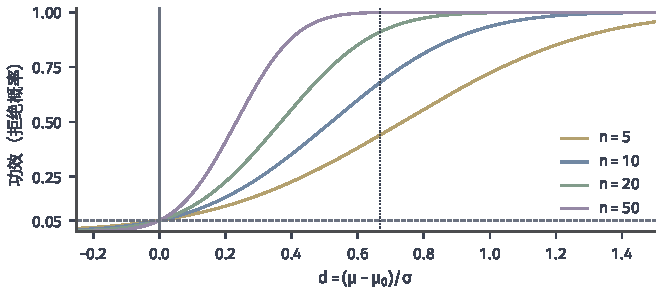
\includegraphics[width=112mm]{figures/01-basic-mathematics/05-probability-and-statistics-basics/matplotlib/pred-power-curves/figure.pdf}
  \caption{$\alpha=0.05$的单侧$z$检验的功效$\Phi(\sqrt n\,d-z_{0.95})$随效应大小$d=(\mu-\mu_0)/\sigma$变化，四条曲线对应$n=5,10,20,50$。$d=0$时所有曲线都等于虚线标出的$\alpha$；$d<0$属于原假设，拒绝概率低于$\alpha$。点线标出$d=2/3$，此处$n=10$的功效约$0.68$，$n=20$约$0.91$。}
  \label{fig:pred-power-curves}
\end{figure}

\begin{example}[功效与样本量]
\label{ex:pred-power-sample-size}
沿用$\sigma=1.5$，检验$H_0:\mu\leq500$，$\alpha=0.05$。若真均值为$501$，则$d=1/1.5\approx0.667$。$n=10$时功效为$\Phi(\sqrt{10}\times0.667-1.645)=\Phi(0.463)\approx0.68$，即约有$32\%$的机会漏掉这$1$ mL的多装。若要求功效达到$0.9$，需要$\sqrt n\,d-z_{0.95}\geq z_{0.9}$，即
\[
 n\geq\Bigl(\frac{z_{0.95}+z_{0.9}}{d}\Bigr)^2=\Bigl(\frac{1.645+1.282}{0.667}\Bigr)^2\approx19.3,
\]
至少需要$20$瓶。这种计算应当在收集数据之前完成。
\end{example}

\paragraph{显著性水平不是结论出错的概率}

$\alpha$是在$H_0$为真的条件下错误拒绝的概率，即$\mathbb P(\text{拒绝}\mid H_0\text{为真})$。人们常常想知道的却是反过来的条件概率：已经拒绝了，$H_0$其实为真的概率是多少？两者一般不相等，后者还取决于被检验的假设中有多少本来就为真。

\begin{example}[拒绝中有多少是错的]
\label{ex:pred-false-rejections}
设某实验室一年做$1000$次检验，其中$900$次$H_0$实际为真，$100$次$H_1$为真；每次检验的水平为$0.05$，在真实效应处的功效为$0.8$。$H_0$为真的$900$次中，约$900\times0.05=45$次被错误拒绝；$H_1$为真的$100$次中，约$80$次被正确拒绝。共拒绝约$125$次，其中$H_0$为真的占$45/125=36\%$，远高于$5\%$。如果真实效应更少或功效更低，这一比例还会更高。
\end{example}

\subsection{$p$值}

\paragraph{定义与计算}

拒绝域给出的是“拒绝”或“不拒绝”二选一的结论，没有说明证据有多强。例~\ref{ex:pred-filling-two-sided}中$t\approx4.19$远超临界值$2.262$，若观测值是$2.3$，结论同样是拒绝，但两者的说服力显然不同。$p$值把“观测结果有多极端”换算为原假设下的尾概率。

\begin{definition}[$p$值]
\label{def:pred-p-value}
设检验统计量$T$的取值越大，越不利于$H_0$。对观测值$t_{\mathrm{obs}}=T(\bm x)$，
\[
 p(\bm x)=\sup_{\theta\in\Theta_0}\mathbb P_\theta\bigl(T(\bm X)\geq t_{\mathrm{obs}}\bigr)
\]
称为\term{$p$值}（$p$-value），即在$H_0$下得到至少与观测结果同样极端的统计量的最大概率。
\end{definition}

定义先要求确定“极端”的顺序，这由$H_1$决定：右侧检验以$T$大为极端；左侧检验可改用$-T$；双侧检验以$|T|$大为极端。$H_0$是简单假设时，上确界就是该点处的尾概率；$H_0$是复合假设时，通常在$\Theta_0$的边界上取到，例如$H_0:\mu\leq500$时取$\mu=500$。

$p$值与拒绝域给出相同的结论：在水平$\alpha$下，$p(\bm x)\leq\alpha$时拒绝$H_0$。以简单原假设、$T$为连续型的情形说明：拒绝域取$R=\{T\geq c\}$，$c$满足$\mathbb P_{\theta_0}(T\geq c)=\alpha$。尾概率$\mathbb P_{\theta_0}(T\geq t)$随$t$递减，所以$t_{\mathrm{obs}}\geq c$当且仅当$\mathbb P_{\theta_0}(T\geq t_{\mathrm{obs}})\leq\alpha$，即$p\leq\alpha$。因此报告$p$值相当于同时报告了所有水平下的结论：$p$值是能够拒绝$H_0$的最小显著性水平。

在同样的条件下还有一个有用的事实：$H_0$为真时，$p$值服从$\operatorname U(0,1)$。记$G(t)=\mathbb P_{\theta_0}(T\geq t)$，则$p=G(T)$；对$0<u<1$，取$c_u$使$G(c_u)=u$，有$\mathbb P_{\theta_0}(G(T)\leq u)=\mathbb P_{\theta_0}(T\geq c_u)=u$。这说明规则“$p\leq\alpha$时拒绝”的第一类错误概率恰为$\alpha$。

\begin{example}[两台灌装机的$p$值]
\label{ex:pred-p-values}
对灌装机A（例~\ref{ex:pred-filling-two-sided}），双侧检验$H_0:\mu=500$的$p$值为
\[
 p=\mathbb P(|T_9|\geq4.19)=2\,\mathbb P(T_9\geq4.19)\approx0.0023,
\]
其中$T_9\sim t_9$。数据与原假设很不相容。

再从灌装机B抽取$8$瓶，灌装量（教学数据）为
\[
 500.2,\ 498.1,\ 501.9,\ 497.6,\ 499.4,\ 502.3,\ 498.8,\ 499.7.
\]
算得$\bar y=499.75$，$s_B\approx1.678$，$t=(499.75-500)/(1.678/\sqrt8)\approx-0.42$。双侧$p$值为$\mathbb P(|T_7|\geq0.42)\approx0.69$，即图~\ref{fig:pred-p-value-tail}中阴影的总面积。在$H_0$下，比这更极端的结果相当常见，数据没有提供否定$H_0$的证据。
\end{example}

\begin{figure}[htbp]
  \centering
  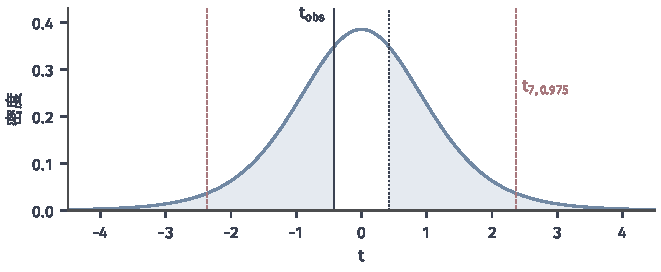
\includegraphics[width=112mm]{figures/01-basic-mathematics/05-probability-and-statistics-basics/matplotlib/pred-p-value-tail/figure.pdf}
  \caption{双侧$p$值是原假设分布的两侧尾面积。曲线为$t_7$分布的密度；实线标出灌装机B的观测值$t_{\mathrm{obs}}\approx-0.42$，点线是它关于零的对称点，两侧阴影面积之和约$0.69$即$p$值。红色虚线是$5\%$水平双侧检验的临界值$\pm t_{7,0.975}\approx\pm2.365$：观测值落在它们之间，相应地$p>0.05$。}
  \label{fig:pred-p-value-tail}
\end{figure}

\paragraph{常见误读}

$p$值是在$H_0$成立的条件下计算出来的，它不是“$H_0$为真的概率”。灌装机A的$p\approx0.0023$不意味着平均灌装量等于$500$的概率是$0.23\%$；后者需要给假设指定先验概率，属于上一节可信区间那一类问题。例~\ref{ex:pred-false-rejections}已经说明，即使$p$值很小，被拒绝的$H_0$中仍可能有相当比例本来为真。

不拒绝$H_0$也不等于证明了$H_0$。灌装机B的$p\approx0.69$只说明数据与$\mu=500$相容；它的$95\%$置信区间是$499.75\pm2.365\times0.593=[498.35,\,501.15]$，与之相容的还有$499$、$501$等许多数值。样本量小、功效低时，即使$H_0$不成立，也很可能不被拒绝。

$p$值的大小也不衡量效应的大小。灌装机A的偏离$\bar x-500=1.5$ mL，约为标称量的$0.3\%$；这一偏离是否重要，取决于成本与规范，而不是$p$值。反过来，若样本量极大，标准误趋于零，再微小的偏离也会给出极小的$p$值。所以报告检验结果时，应当同时报告估计值和置信区间：前者说明效应多大，后者说明估计有多精确。

\subsection{单总体均值检验}

\paragraph{统计量的选择}

前面的例子已经用过均值检验。系统地说，检验$\mu=\mu_0$所用的统计量与第~\ref{sec:pred-intervals}节的区间完全平行，按总体条件分三种情形：
\begin{center}
\begin{tabular}{lll}
  \toprule
  总体条件 & 统计量 & $H_0$下的分布\\
  \midrule
  正态，$\sigma$已知 & $Z=\dfrac{\bar X-\mu_0}{\sigma/\sqrt n}$ & $\mathcal N(0,1)$，精确\\[1.2ex]
  正态，$\sigma$未知 & $T=\dfrac{\bar X-\mu_0}{S/\sqrt n}$ & $t_{n-1}$，精确\\[1.2ex]
  独立同分布，方差有限 & $T=\dfrac{\bar X-\mu_0}{S/\sqrt n}$ & 近似$\mathcal N(0,1)$，$n$大时\\
  \bottomrule
\end{tabular}
\end{center}
第二种称为单样本\term{$t$检验}（$t$ test）。第三种情形的水平只在渐近意义下成立，例~\ref{ex:pred-exponential-coverage}中偏斜总体的覆盖不足，同样会表现为单侧检验的实际水平偏离名义值。

\paragraph{单侧与双侧拒绝域}

统计量确定之后，拒绝域的位置由备择假设决定。我们用灌装机A的数据，把同一个统计量放进三种检验问题中比较。

\begin{example}[灌装量的三种检验]
\label{ex:pred-filling-three-tests}
对例~\ref{ex:pred-filling-data}，$t\approx4.19$，自由度$9$，$\alpha=0.05$：
\begin{itemize}
  \item $H_1:\mu\neq500$：拒绝域$|t|>2.262$，$p=2\,\mathbb P(T_9\geq4.19)\approx0.0023$，拒绝；
  \item $H_1:\mu>500$：拒绝域$t>t_{9,0.95}=1.833$，$p=\mathbb P(T_9\geq4.19)\approx0.0012$，拒绝；
  \item $H_1:\mu<500$：拒绝域$t<-1.833$，$p=\mathbb P(T_9\leq4.19)\approx0.9988$，不拒绝。
\end{itemize}
同侧的单侧检验的临界值比双侧小，$p$值是双侧的一半，因为全部$\alpha$都放在了一侧。但这只在方向事先确定时才合理；看到$\bar x>500$之后再选择右侧检验，相当于把双侧检验的$p$值减半，实际水平会翻倍。
\end{example}

检验结论应与估计一起解释。这批数据的结论是：平均灌装量显著高于$500$ mL（$p\approx0.002$），估计多装$1.5$ mL，$95\%$置信区间为$[0.69,\,2.31]$ mL。以样本标准差为单位，偏离约为$1.5/1.13\approx1.3$个标准差，相对于瓶间波动并不算小；但相对于$500$ mL的总量只占约$0.3\%$。是否需要调整设备，取决于多装的成本与质量规范。

\subsection{两总体均值比较}

\paragraph{独立两组与配对数据}

比较两个总体的均值时，首先要看数据是怎样收集的。若两组观测分别来自不同的个体，例如从灌装机A、B各自抽瓶，两组相互独立，称为独立样本；若每个个体被测量两次，例如同一件样品分别用新旧两种方法测量，两次测量成对出现，称为配对数据。配对数据中，同一样品的两次测量共享样品自身的特性，因而相关；把它们当作两个独立组来分析，会把样品之间的差异混入比较。

配对数据的处理很简单：对每一对取差值$D_i=V_i-U_i$，问题就变为差值总体的均值$\mu_D$是否为零，即单总体均值检验。假设$D_1,\dots,D_n$独立同分布于正态总体，统计量$T=\bar D/(S_D/\sqrt n)$在$H_0:\mu_D=0$下服从$t_{n-1}$，这称为配对$t$检验。

\begin{example}[配对设计与错误的独立分析]
\label{ex:pred-paired}
$8$件样品分别用旧方法$u_i$与新方法$v_i$测量某成分含量（单位：mg，教学数据）：
\begin{center}
\begin{tabular}{lcccccccc}
  \toprule
  样品 & 1 & 2 & 3 & 4 & 5 & 6 & 7 & 8\\
  \midrule
  旧方法$u_i$ & 12.4 & 15.1 & 9.8 & 14.2 & 11.6 & 13.0 & 10.5 & 12.9\\
  新方法$v_i$ & 12.9 & 15.3 & 10.6 & 14.5 & 11.8 & 13.7 & 10.8 & 13.4\\
  差值$d_i$ & 0.5 & 0.2 & 0.8 & 0.3 & 0.2 & 0.7 & 0.3 & 0.5\\
  \bottomrule
\end{tabular}
\end{center}
差值的均值$\bar d=3.5/8=0.4375$，标准差$s_D\approx0.226$，于是$t=0.4375/(0.226/\sqrt8)\approx5.47$，自由度$7$，双侧$p\approx0.0009$；$\mu_D$的$95\%$置信区间为$0.4375\pm2.365\times0.080=[0.25,\,0.63]$。新方法系统地偏高约$0.44$ mg。

若错误地把两列当作独立样本，用下文的合并方差$t$检验，得到$p\approx0.62$，看不出任何差异。原因在于样品之间含量差异很大（从约$10$到约$15$ mg），独立分析把这部分差异算作噪声；取差值后，同一样品的特性相互抵消，只剩下方法差异和测量误差。
\end{example}

\paragraph{合并方差$t$检验}

再来看独立样本。设$X_1,\dots,X_{n_1}$独立同分布于$\mathcal N(\mu_1,\sigma^2)$，$Y_1,\dots,Y_{n_2}$独立同分布于$\mathcal N(\mu_2,\sigma^2)$，两组相互独立。这里的关键假设是\emph{两总体方差相等}。检验$H_0:\mu_1=\mu_2$。

我们仿照单样本情形构造枢轴量。由独立性，$\bar X-\bar Y\sim\mathcal N\bigl(\mu_1-\mu_2,\ \sigma^2(1/n_1+1/n_2)\bigr)$。两组的样本方差都估计同一个$\sigma^2$，把它们按自由度加权合并：
\[
 S_p^2=\frac{(n_1-1)S_X^2+(n_2-1)S_Y^2}{n_1+n_2-2}.
\]
由第~\ref{sec:samp-chi-square}节，$(n_1-1)S_X^2/\sigma^2\sim\chi^2_{n_1-1}$，$(n_2-1)S_Y^2/\sigma^2\sim\chi^2_{n_2-1}$，二者独立。卡方变量是独立标准正态变量的平方和，两个独立卡方变量相加，相当于把两组独立标准正态变量合在一起求平方和，所以$(n_1+n_2-2)S_p^2/\sigma^2\sim\chi^2_{n_1+n_2-2}$。它又与$\bar X-\bar Y$独立，因为每组内样本均值与样本方差独立，两组之间也独立。按$t$分布的定义（第~\ref{sec:samp-t}节），
\begin{equation}
 T=\frac{(\bar X-\bar Y)-(\mu_1-\mu_2)}{S_p\sqrt{1/n_1+1/n_2}}\sim t_{n_1+n_2-2}.
 \label{eq:pred-pooled-t}
\end{equation}
令$\mu_1-\mu_2=0$即得检验统计量，称为合并方差$t$检验；反解$T$也得到$\mu_1-\mu_2$的置信区间。

\begin{example}[两台灌装机的比较]
\label{ex:pred-two-machines}
灌装机A（例~\ref{ex:pred-filling-data}）：$n_1=10$，$\bar x=501.5$，$s_X^2\approx1.282$；灌装机B（例~\ref{ex:pred-p-values}）：$n_2=8$，$\bar y=499.75$，$s_Y^2\approx2.814$。合并方差
\[
 s_p^2=\frac{9\times1.282+7\times2.814}{16}=\frac{11.54+19.70}{16}\approx1.953,
\]
标准误$s_p\sqrt{1/10+1/8}\approx0.663$，$t=1.75/0.663\approx2.64$，自由度$16$，双侧$p\approx0.018$。$\mu_1-\mu_2$的$95\%$置信区间为$1.75\pm2.120\times0.663=[0.34,\,3.16]$。
\end{example}

\paragraph{Welch方法}

等方差是一个实质性的假设。上例中两组样本方差相差一倍以上，等方差未必成立。若两总体方差不等而样本量又不同，合并方差会把两组的波动按错误的权重混合，$T$的实际分布偏离$t_{n_1+n_2-2}$，检验水平可能明显失真。

不假设等方差时，自然的做法是分别估计两组的方差：
\[
 T_W=\frac{\bar X-\bar Y}{\sqrt{S_X^2/n_1+S_Y^2/n_2}}.
\]
这时$T_W$在$H_0$下不再精确服从任何$t$分布，但可以用一个$t$分布近似，其自由度由Welch--Satterthwaite公式给出：
\[
 \nu=\frac{\bigl(S_X^2/n_1+S_Y^2/n_2\bigr)^2}{\dfrac{(S_X^2/n_1)^2}{n_1-1}+\dfrac{(S_Y^2/n_2)^2}{n_2-1}}.
\]
这个公式的想法是：选择$\nu$，使$\nu\cdot(S_X^2/n_1+S_Y^2/n_2)/(\sigma_1^2/n_1+\sigma_2^2/n_2)$的前两阶矩与$\chi^2_\nu$相同，再把未知方差换成样本方差。所得的\term{Welch检验}（Welch test）是近似方法，但在两总体方差相等与否时都表现良好，因此当没有充分理由相信等方差时，通常默认使用它。

\begin{example}[两台灌装机的Welch检验]
\label{ex:pred-welch}
续例~\ref{ex:pred-two-machines}，$s_X^2/n_1\approx0.128$，$s_Y^2/n_2\approx0.352$，标准误$\sqrt{0.128+0.352}\approx0.693$，$t_W=1.75/0.693\approx2.53$，自由度$\nu\approx11.8$，双侧$p\approx0.027$。结论与合并方差检验相同，但标准误略大、自由度更小，证据显得稍弱。
\end{example}

\subsection{比例检验}

\paragraph{精确二项检验}

合同规定封口不合格率不得超过$5\%$。抽查$40$瓶发现$6$瓶不合格（例~\ref{ex:pred-wald}），能否认定不合格率超标？检验问题为$H_0:p\leq0.05$，$H_1:p>0.05$。

不合格数$S\sim\operatorname{Bin}(40,p)$，$S$越大越不利于$H_0$，拒绝域取右尾$\{S\geq c\}$。按第~\ref{sec:pred-intervals}节证明的单调性，$\mathbb P_p(S\geq c)$随$p$增加，因此$\Theta_0=[0,0.05]$上的最大拒绝概率在边界$p=0.05$处取到，只需在$\operatorname{Bin}(40,0.05)$下计算。$H_0$下的尾概率为
\[
 \mathbb P(S\geq4)\approx0.138,\qquad\mathbb P(S\geq5)\approx0.048,\qquad\mathbb P(S\geq6)\approx0.014.
\]
要使水平不超过$0.05$，最小的临界值是$c=5$，拒绝域为$\{S\geq5\}$，实际水平为$0.048$。观测值$s=6$落入拒绝域，$p$值为$\mathbb P(S\geq6)\approx0.014$，拒绝$H_0$。

这里实际水平$0.048$略低于名义值$0.05$，这又是离散性的结果：$S$只取整数，尾概率只能取有限个值，一般无法恰好等于$\alpha$。若取$c=4$，水平升至$0.138$，超出要求。所以精确二项检验通常是保守的，这与Clopper--Pearson区间的保守覆盖出自同一原因。

双侧问题$H_0:p=p_0$还需决定怎样合并两侧尾部。常用做法是计算观测值所在一侧的尾概率并乘以$2$（不超过$1$）；由于二项分布在$p_0\neq1/2$时不对称，不同的合并方式可能给出不同的$p$值，报告时应说明所用方法。

\paragraph{正态近似}

样本量较大时，可以用正态分布近似$S$。$H_0:p=p_0$下$\hat p$的均值为$p_0$、方差为$p_0(1-p_0)/n$，统计量
\[
 Z=\frac{\hat p-p_0}{\sqrt{p_0(1-p_0)/n}}
\]
近似服从$\mathcal N(0,1)$。注意分母使用的是原假设下的$p_0$，而不是$\hat p$：检验在$H_0$成立的前提下计算统计量的分布，方差应按$H_0$来算。

\begin{example}[精确计算与正态近似的比较]
\label{ex:pred-binomial-approx}
对$n=40$、$s=6$、$p_0=0.05$，$\hat p=0.15$，$Z=(0.15-0.05)/\sqrt{0.05\times0.95/40}\approx2.90$，近似$p$值为$1-\Phi(2.90)\approx0.0019$，只有精确值$0.014$的约七分之一。图~\ref{fig:pred-binomial-test}说明了原因：$np_0=2$，二项分布明显右偏，正态曲线的右尾下降得比真实概率快得多。这里结论碰巧相同。若观测值是$s=5$，精确$p$值为$0.048$，刚好在$5\%$水平下拒绝；近似$p$值约为$0.015$，又一次把证据夸大了约三倍。在更接近临界的情形中，这种夸大足以改变结论。
\end{example}

\begin{figure}[htbp]
  \centering
  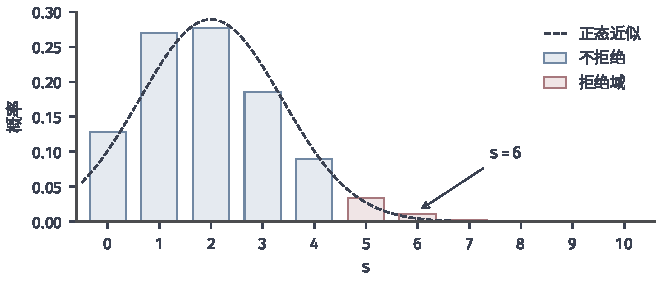
\includegraphics[width=112mm]{figures/01-basic-mathematics/05-probability-and-statistics-basics/matplotlib/pred-binomial-test/figure.pdf}
  \caption{原假设$p=0.05$下不合格数$S\sim\operatorname{Bin}(40,0.05)$的概率。红色柱为$5\%$水平的拒绝域$\{S\geq5\}$，总概率约$0.048$；箭头标出观测值$s=6$，其右尾概率约$0.014$即精确$p$值。虚线是均值$2$、方差$1.9$的正态近似密度，它在右尾明显低于二项概率，因而低估了$p$值。}
  \label{fig:pred-binomial-test}
\end{figure}

一个常用的经验规则是：$np_0$与$n(1-p_0)$都至少约为$10$时，正态近似才比较可靠。这是经验判断，不是定理；可以计算精确值时，应优先使用精确的二项检验。

\subsection{方差检验}

\paragraph{单个正态总体}

设备规范要求灌装量的标准差不超过$1.5$ mL。对正态样本，检验$H_0:\sigma^2=\sigma_0^2$用第~\ref{sec:pred-intervals}节的卡方枢轴量，在$H_0$下
\[
 \chi^2=\frac{(n-1)S^2}{\sigma_0^2}\sim\chi^2_{n-1}.
\]
双侧检验的拒绝域为$\{\chi^2<\chi^2_{n-1,\alpha/2}\}\cup\{\chi^2>\chi^2_{n-1,1-\alpha/2}\}$；关心方差是否过大时，用右侧拒绝域$\{\chi^2>\chi^2_{n-1,1-\alpha}\}$。

\begin{example}[灌装量的方差检验]
\label{ex:pred-variance-test}
对例~\ref{ex:pred-filling-data}检验$H_0:\sigma=1.5$，$\chi^2=11.54/2.25\approx5.13$。双侧$5\%$水平的拒绝域是$\chi^2<2.700$或$\chi^2>19.023$，观测值不在其中，双侧$p\approx0.35$。若只关心波动是否过大，$H_1:\sigma>1.5$，则观测值在分布的左侧，更没有理由拒绝。这与例~\ref{ex:pred-filling-variance-interval}中$\sigma$的区间$[0.779,\,2.067]$包含$1.5$是一致的。
\end{example}

和方差区间一样，这个检验的水平完全依赖正态性；总体尾部较厚时，检验会过多地拒绝，并且不因样本量增大而改善。

\paragraph{两个正态总体的$F$检验}

比较两台灌装机的波动，检验$H_0:\sigma_1^2=\sigma_2^2$。设两组独立，各自来自正态总体。$(n_1-1)S_X^2/\sigma_1^2$与$(n_2-1)S_Y^2/\sigma_2^2$分别服从$\chi^2_{n_1-1}$、$\chi^2_{n_2-1}$且相互独立，按第~\ref{sec:samp-f}节$F$分布的定义，
\[
 \frac{S_Y^2/\sigma_2^2}{S_X^2/\sigma_1^2}\sim F_{n_2-1,\,n_1-1}.
\]
$H_0$下$\sigma_1^2=\sigma_2^2$相消，统计量$F=S_Y^2/S_X^2\sim F_{n_2-1,n_1-1}$，比值过大或过小都不利于$H_0$。

\begin{example}[两台灌装机的方差比较]
\label{ex:pred-f-test}
续例~\ref{ex:pred-two-machines}，$F=2.814/1.282\approx2.19$，自由度$(7,9)$。$F_{7,9,0.025}\approx0.207$，$F_{7,9,0.975}\approx4.197$，观测值落在两者之间，双侧$p\approx0.27$，不拒绝等方差假设。
\end{example}

这个结果不能读作“两台机器的方差相等”。两组各只有十个左右的观测，方差比的估计很粗糙，即使真实方差相差一倍，$F$检验也很可能不拒绝。正因如此，不宜先用$F$检验判断等方差、再据此在合并方差与Welch方法之间选择；直接使用Welch方法更稳妥。此外，$F$检验对非正态性同样敏感，原因与卡方检验相同。

\subsection{检验与置信区间的关系}

\paragraph{由检验族构造置信集合}

例~\ref{ex:pred-variance-test}中，检验不拒绝$\sigma=1.5$，而$\sigma$的置信区间恰好包含$1.5$，这不是巧合。对每一个可能的参数值$\theta_0$，都可以检验$H_0:\theta=\theta_0$；把所有未被拒绝的$\theta_0$收集起来，就得到一个置信集合。

\begin{theorem}[检验与置信集合的对偶]
\label{thm:pred-test-interval-duality}
设对每个$\theta_0\in\Theta$，都有$H_0:\theta=\theta_0$的水平为$\alpha$的检验，把它的拒绝域直接写成样本的集合$R(\theta_0)$，即$\mathbb P_{\theta_0}\bigl(\bm X\in R(\theta_0)\bigr)\leq\alpha$。令
\[
 C(\bm X)=\{\theta_0\in\Theta:\bm X\notin R(\theta_0)\},
\]
则对每个$\theta\in\Theta$，$\mathbb P_\theta\bigl(\theta\in C(\bm X)\bigr)\geq1-\alpha$。反过来，若$C(\bm X)$是置信水平为$1-\alpha$的置信集合（即把定义~\ref{def:pred-confidence-interval}中的区间换成一般的参数集合），则“$\theta_0\notin C(\bm X)$时拒绝”是$H_0:\theta=\theta_0$的水平为$\alpha$的检验。
\end{theorem}

\begin{proof}
由$C$的定义，$\theta\in C(\bm X)$当且仅当$\bm X\notin R(\theta)$。故$\mathbb P_\theta\bigl(\theta\in C(\bm X)\bigr)=1-\mathbb P_\theta\bigl(\bm X\in R(\theta)\bigr)\geq1-\alpha$。反方向，拒绝域为$\{\bm X:\theta_0\notin C(\bm X)\}$，其在$\theta_0$下的概率为$1-\mathbb P_{\theta_0}\bigl(\theta_0\in C(\bm X)\bigr)\leq\alpha$。
\end{proof}

定理说明，“检验”和“置信集合”是同一族事件$\{\bm X\notin R(\theta_0)\}$的两种读法：固定$\theta_0$看哪些样本会拒绝它，得到检验；固定样本看哪些$\theta_0$未被拒绝，得到置信集合。定理给出的置信集合不一定是区间，但在常见的单参数问题中通常是。

\paragraph{均值双侧检验的对应}

以$t$检验为例。水平$\alpha$的双侧$t$检验在$|\bar x-\mu_0|/(s/\sqrt n)\leq t_{n-1,1-\alpha/2}$时不拒绝$H_0:\mu=\mu_0$，这个不等式对$\mu_0$解出来就是
\[
 \bar x-t_{n-1,1-\alpha/2}\frac s{\sqrt n}\leq\mu_0\leq\bar x+t_{n-1,1-\alpha/2}\frac s{\sqrt n},
\]
恰好是$t$区间~\eqref{eq:pred-t-interval}。所以对灌装机A，$500$不在$95\%$区间$[500.69,\,502.31]$中，等价于$5\%$水平的双侧$t$检验拒绝$\mu=500$。图~\ref{fig:pred-test-interval-duality}把双侧$p$值看作$\mu_0$的函数：曲线在$\bar x$处达到$1$，向两侧下降；$p$值高于$0.05$的$\mu_0$恰好组成$95\%$置信区间。

\begin{figure}[htbp]
  \centering
  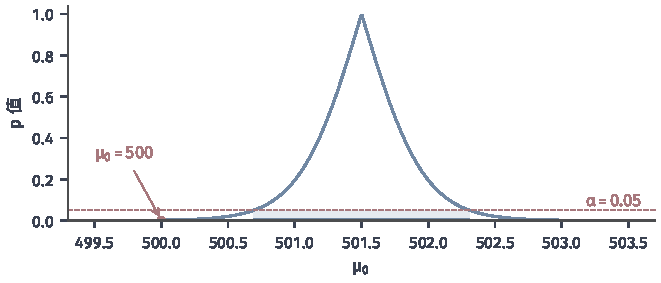
\includegraphics[width=112mm]{figures/01-basic-mathematics/05-probability-and-statistics-basics/matplotlib/pred-test-interval-duality/figure.pdf}
  \caption{灌装机A数据的双侧$t$检验$p$值作为待检验值$\mu_0$的函数，$p(\mu_0)=2\,\mathbb P\bigl(T_9\geq|\bar x-\mu_0|/(s/\sqrt{10})\bigr)$。红色虚线为$\alpha=0.05$；曲线在虚线之上的$\mu_0$不被拒绝，它们构成横轴上加粗标出的$95\%$置信区间$[500.69,\,502.31]$。红点为$\mu_0=500$，$p\approx0.0023$，位于区间外。}
  \label{fig:pred-test-interval-duality}
\end{figure}

这种对应要求区间与检验由同一族构造得到：相同的统计量、相同的标准误、相同的尾部规则。若两者不匹配，就不能直接用区间判断检验结果。

\begin{example}[不匹配的区间与检验]
\label{ex:pred-mismatch}
单侧检验对应单侧置信界，而不是双侧区间。灌装机A的右侧检验$H_1:\mu>500$对应置信下界$\bar x-t_{9,0.95}\,s/\sqrt{10}\approx500.84$：$500$低于它，故拒绝。若改用双侧$95\%$区间判断单侧检验，实际相当于在$2.5\%$水平下检验。

比例问题中的不匹配更明显。对$n=40$、$s=6$，Wald区间$[0.039,\,0.261]$包含$0.05$；但例~\ref{ex:pred-binomial-approx}中的正态近似检验给出$Z\approx2.90$，强烈拒绝$p=0.05$。两者的标准误不同：Wald区间用$\sqrt{\hat p(1-\hat p)/n}\approx0.056$，检验用$\sqrt{p_0(1-p_0)/n}\approx0.034$。由这个检验族反解得到的区间，即把$|\hat p-p_0|\leq z_{0.975}\sqrt{p_0(1-p_0)/n}$对$p_0$解出的二次不等式的解集，约为$[0.071,\,0.291]$，它不包含$0.05$，与检验结论一致。
\end{example}

\section{未来观测的预测}
\label{sec:pred-prediction}

前两节的对象都是参数，它是总体的一个固定特征。质检员还关心另一类问题：下一瓶会装多少？这时要猜测的是一个尚未发生的随机结果，即使参数完全已知，也不可能准确猜中。本节先明确预测的对象和点预测的标准，再分析预测误差的来源，然后在正态模型中构造预测区间，最后用后验分布给出另一种预测方式。

\subsection{预测对象与点预测}

\paragraph{三种不同的对象}

在灌装的例子里，至少有三种量都可以称为“估计灌装量”：总体均值$\mu$，这是参数；下一瓶的灌装量$X_{n+1}$，这是单个未来观测；下一批$m$瓶的平均灌装量$\bar X'_m$，这是未来观测的汇总量。三者都可以用同一个数$\bar x=501.5$去猜，但猜测的误差完全不同。

设未来观测与已有样本独立同分布，方差为$\sigma^2$。参数$\mu$固定不动，误差只来自估计；$X_{n+1}$本身围绕$\mu$以方差$\sigma^2$波动；$\bar X'_m$的方差为$\sigma^2/m$，介于二者之间。$m=1$时它就是单个观测，$m\to\infty$时它趋于参数。所以说明“预测什么”是第一步：对象改变后，误差的含义和大小都随之改变。

\paragraph{平方误差下的最优点预测}

先只用一个数来预测随机变量$Y$。若用常数$c$，并以平方误差$(Y-c)^2$衡量损失，设$\mathbb E Y^2<\infty$，则
\begin{equation}
 \mathbb E(Y-c)^2=\mathbb E\bigl((Y-\mathbb EY)+(\mathbb EY-c)\bigr)^2=\operatorname{Var}(Y)+(\mathbb EY-c)^2,
 \label{eq:pred-mse-constant}
\end{equation}
交叉项$2(\mathbb EY-c)\,\mathbb E(Y-\mathbb EY)=0$。右边第一项与$c$无关，第二项在$c=\mathbb EY$时为零，所以均值是平方误差下的最优常数预测，最小误差就是方差。

若预测时还能观测到另一个变量$X$，预测可以写成$X$的函数$g(X)$。第~\ref{sec:rvec-conditional-expectation}节的条件期望$r(X)=\mathbb E(Y\mid X)$满足：对任何$X$的函数$h(X)$（使下式中的期望有限），$\mathbb E\bigl[(Y-r(X))h(X)\bigr]=0$。这可以由塔性质$\mathbb E\bigl[\mathbb E(Y\mid X)h(X)\bigr]=\mathbb E[Yh(X)]$得到。取$h=r-g$，与式~\eqref{eq:pred-mse-constant}同样展开，交叉项消失：
\begin{equation}
 \mathbb E\bigl(Y-g(X)\bigr)^2=\mathbb E\bigl(Y-r(X)\bigr)^2+\mathbb E\bigl(r(X)-g(X)\bigr)^2.
 \label{eq:pred-mse-conditional}
\end{equation}
因此在有限二阶矩条件下，条件均值$\mathbb E(Y\mid X)$是平方误差意义下的最优预测，第一项是任何预测都无法消除的误差。第~\ref{sec:pred-regression}节的回归函数$\beta_0+\beta_1x$正是一个条件均值的模型。

最优预测依赖于损失的选择。若改用绝对误差$|Y-c|$，最优常数是中位数而不是均值。

\begin{example}[均值与中位数作为预测]
\label{ex:pred-mean-median}
设某商品每日退货数$Y$取$0,1,10$，概率分别为$0.5,0.3,0.2$。$\mathbb EY=0.3+2=2.3$，平方误差下最优预测是$2.3$，最小均方误差为$\operatorname{Var}(Y)=\mathbb EY^2-2.3^2=20.3-5.29=15.01$。若按绝对误差，预测值$c\in[0,1]$时期望损失为$0.5c+0.3(1-c)+0.2(10-c)=2.3$，与$c$无关，区间$[0,1]$中的每个点都是中位数，也都是最优预测；而用$2.3$时期望绝对误差为$0.5\times2.3+0.3\times1.3+0.2\times7.7=3.08$。罕见的大值把均值拉高，中位数则不受影响。
\end{example}

\subsection{预测误差的来源}

\paragraph{参数已知时}

回到正态位置模型：$X_1,\dots,X_n,X_{n+1}$独立同分布于$\mathcal N(\mu,\sigma^2)$，要用前$n$个观测预测$X_{n+1}$。先设想$\mu$已知。由上一小节，最优点预测是$\mu$，预测误差$X_{n+1}-\mu\sim\mathcal N(0,\sigma^2)$。这部分误差来自新观测自身的随机波动，与历史数据的多少无关，称为不可约误差。即使知道总体的一切，也无法消除它。

\paragraph{参数需要估计时}

实际中$\mu$未知，只能用$\bar X$代替。预测误差变为
\[
 X_{n+1}-\bar X=(X_{n+1}-\mu)-(\bar X-\mu).
\]
第一项是新观测的波动，第二项是估计参数带来的误差。由于$X_{n+1}$与$X_1,\dots,X_n$独立，两项独立，方差相加：
\begin{equation}
 \mathbb E(X_{n+1}-\bar X)^2=\operatorname{Var}(X_{n+1}-\bar X)=\sigma^2+\frac{\sigma^2}n=\sigma^2\Bigl(1+\frac1n\Bigr).
 \label{eq:pred-prediction-variance}
\end{equation}
这里第一个等号用到$\mathbb E(X_{n+1}-\bar X)=0$。这个结论只需要独立同分布与有限方差，不需要正态性。

\begin{example}[两种误差的相对大小]
\label{ex:pred-error-sources}
取$\sigma=1.5$，$n=10$。新观测的波动贡献$\sigma^2=2.25$，参数估计贡献$\sigma^2/n=0.225$，总预测均方误差$2.475$，其中参数误差只占约$9\%$。把样本量增至$100$，参数误差降为$0.0225$，总误差$2.2725$，只减少了约$8\%$。增加历史数据很快就无法再改善单瓶的预测。
\end{example}

\subsection{正态位置模型的预测区间}

\paragraph{精确预测区间}

点预测之外，我们希望给出一个区间，使下一瓶的灌装量以指定概率落在其中。

\begin{definition}[预测区间]
\label{def:pred-prediction-interval}
设$L(\bm X)\leq U(\bm X)$是样本$\bm X=(X_1,\dots,X_n)$的统计量，$Y$是尚未观测的随机变量。若对模型中的每个参数，
\[
 \mathbb P\bigl(L(\bm X)\leq Y\leq U(\bm X)\bigr)\geq1-\alpha,
\]
则称$[L(\bm X),U(\bm X)]$为$Y$的水平为$1-\alpha$的\term{预测区间}（prediction interval）。这里的概率对样本$\bm X$与未来观测$Y$联合计算。
\end{definition}

与置信区间相比，被覆盖的对象从固定参数变成了随机变量，概率也同时包含了样本和新观测两部分随机性。

在正态位置模型中，由式~\eqref{eq:pred-prediction-variance}，$X_{n+1}-\bar X\sim\mathcal N\bigl(0,\sigma^2(1+1/n)\bigr)$，它是独立正态变量的线性组合，因而仍是正态的。为了处理未知的$\sigma$，再用$S$代替它。$X_{n+1}$与$(\bar X,S^2)$独立，因为后者只依赖$X_1,\dots,X_n$；又由第~\ref{sec:samp-normal}节，$\bar X$与$S^2$独立。所以$X_{n+1}$、$\bar X$、$S^2$三者相互独立，$X_{n+1}-\bar X$作为前两者的函数与$S^2$独立。按$t$分布的定义，
\[
 \frac{X_{n+1}-\bar X}{S\sqrt{1+1/n}}
 =\frac{(X_{n+1}-\bar X)\big/\bigl(\sigma\sqrt{1+1/n}\bigr)}{\sqrt{\dfrac{(n-1)S^2/\sigma^2}{n-1}}}
 \sim t_{n-1}.
\]
它的分布不含未知参数，反解得到$X_{n+1}$的预测区间
\begin{equation}
 \bar X\pm t_{n-1,1-\alpha/2}\,S\sqrt{1+\frac1n}.
 \label{eq:pred-normal-prediction-interval}
\end{equation}
对正态总体，其覆盖概率恰为$1-\alpha$。

\begin{example}[下一瓶的预测区间]
\label{ex:pred-filling-prediction}
对例~\ref{ex:pred-filling-data}，$95\%$预测区间为
\[
 501.5\pm2.262\times1.1324\times\sqrt{1.1}=501.5\pm2.687=[498.81,\,504.19].
\]
它比均值的$t$区间$[500.69,\,502.31]$宽约$3.3$倍。前者说的是下一瓶，后者说的是平均灌装量。
\end{example}

\paragraph{两种宽度的比较}

把预测区间~\eqref{eq:pred-normal-prediction-interval}与均值区间~\eqref{eq:pred-t-interval}放在一起看，两者的中心相同，分位数相同，只有半宽中的因子不同：均值区间是$1/\sqrt n$，预测区间是$\sqrt{1+1/n}$，比值为$\sqrt{n+1}$。$n\to\infty$时，$1/\sqrt n\to0$，均值区间收缩到一个点；$\sqrt{1+1/n}\to1$，预测区间趋于$\mu\pm z_{1-\alpha/2}\sigma$，这正是参数已知时新观测的波动范围。图~\ref{fig:pred-interval-widths}以$\sigma$已知的情形画出了这两条曲线：增加样本可以消除参数误差，但无法消除新观测的噪声。

\begin{figure}[htbp]
  \centering
  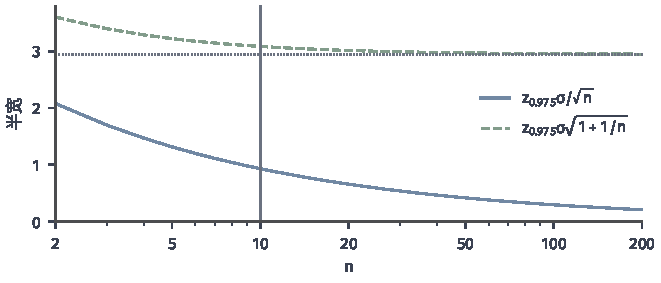
\includegraphics[width=112mm]{figures/01-basic-mathematics/05-probability-and-statistics-basics/matplotlib/pred-interval-widths/figure.pdf}
  \caption{$\sigma=1.5$已知时，$95\%$均值置信区间与预测区间的半宽随样本量$n$变化（横轴为对数刻度）。蓝实线$1.96\sigma/\sqrt n$趋于零；绿虚线$1.96\sigma\sqrt{1+1/n}$趋于点线标出的极限$1.96\sigma\approx2.94$。竖线标出$n=10$，此时两者分别约为$0.93$与$3.08$。}
  \label{fig:pred-interval-widths}
\end{figure}

预测区间对正态性的依赖比均值区间更强。均值区间在非正态总体下还有中心极限定理的大样本保证，因为$\bar X$是许多观测的平均；预测区间要覆盖的却是单个观测$X_{n+1}$，它的分布就是总体分布本身，不会因为$n$增大而变得接近正态。若总体偏斜或厚尾，式~\eqref{eq:pred-normal-prediction-interval}的覆盖率即使在大样本下也可能偏离名义值。这时可以改用基于样本分位数等不依赖分布形式的方法，相关内容见\BookChapterRef{chap:statistical-inference}{卷4《数学准备：流形、概率分布与统计推断》的“统计推断”章}。

\subsection{后验预测}

\paragraph{后验预测分布}

在贝叶斯框架中，参数的不确定性已由后验分布描述，预测可以直接由它推出。设给定参数$\theta$时，未来观测$Y$与已有样本$\bm X$条件独立，$Y$的密度（或质量函数）为$f(y\mid\theta)$。对后验分布求平均，
\begin{equation}
 f(y\mid\bm x)=\int_\Theta f(y\mid\theta)\,\pi(\theta\mid\bm x)\,\mathrm d\theta,
 \label{eq:pred-posterior-predictive}
\end{equation}
其中$\pi(\theta\mid\bm x)$是后验密度；参数离散时积分换成求和。这一分布称为\term{后验预测分布}（posterior predictive distribution）。它的推导就是全概率公式：$Y$与$\theta$在给定$\bm x$下的联合密度为$f(y\mid\theta,\bm x)\pi(\theta\mid\bm x)$，由条件独立性，$f(y\mid\theta,\bm x)=f(y\mid\theta)$，再对$\theta$积分即得边缘密度。

式~\eqref{eq:pred-posterior-predictive}中有两层不确定性：被积函数$f(y\mid\theta)$描述参数给定时新观测的波动，权重$\pi(\theta\mid\bm x)$描述参数本身的不确定性。这与前面分析的两种预测误差来源一一对应。与之相比，直接把点估计$\hat\theta$代入$f(y\mid\hat\theta)$的“代入预测”只保留了第一层，因而低估了预测的不确定性。

\paragraph{Beta--Bernoulli模型}

在Beta--Bernoulli模型中，下一瓶是否不合格$X_{n+1}\in\{0,1\}$，给定$p$时$\mathbb P(X_{n+1}=1\mid p)=p$。由式~\eqref{eq:pred-posterior-predictive}，
\[
 \mathbb P(X_{n+1}=1\mid\bm x)=\int_0^1p\,\pi(p\mid\bm x)\,\mathrm dp=\mathbb E(p\mid\bm x)=\frac{a+s}{a+b+n},
\]
最后一步用到$\operatorname{Beta}(a+s,b+n-s)$的均值。下一次成功的预测概率就是后验均值。

\begin{example}[下一瓶不合格的概率]
\label{ex:pred-beta-predictive}
续例~\ref{ex:pred-beta-credible}，均匀先验下，$40$瓶中$6$瓶不合格，下一瓶不合格的后验预测概率为$(1+6)/(2+40)=1/6\approx0.167$，略高于样本比例$0.15$。若$20$瓶全部合格，后验预测概率为$1/22\approx0.045$，而不是代入$\hat p=0$得到的$0$。均匀先验相当于事先多看了一次成功和一次失败，使预测不会因为尚未见过某种结果就断言它不可能发生。
\end{example}

\paragraph{高斯均值模型}

在例~\ref{ex:pred-normal-credible}的模型中，$\sigma^2$已知，$\mu$的后验为$\mathcal N(\mu_n,\tau_n^2)$。新观测可以写成$X_{n+1}=\mu+\varepsilon$，其中在给定数据下$\mu\sim\mathcal N(\mu_n,\tau_n^2)$，$\varepsilon\sim\mathcal N(0,\sigma^2)$，且二者独立。独立正态变量之和仍为正态，均值与方差分别相加，所以后验预测分布为
\begin{equation}
 X_{n+1}\mid\bm x\sim\mathcal N\bigl(\mu_n,\ \sigma^2+\tau_n^2\bigr).
 \label{eq:pred-normal-posterior-predictive}
\end{equation}
预测方差中$\sigma^2$是观测噪声，$\tau_n^2$是参数后验的方差。$n\to\infty$时$\tau_n^2\to0$，预测方差趋于$\sigma^2$，与频率学派预测区间的极限一致。

\begin{example}[下一瓶的后验预测区间]
\label{ex:pred-normal-predictive}
续例~\ref{ex:pred-normal-credible}，$\mu_n\approx501.22$，$\tau_n^2\approx0.184$，$\sigma^2=2.25$。预测方差$2.25+0.184=2.434$，标准差约$1.560$，$95\%$后验预测区间为$501.22\pm1.96\times1.560=[498.17,\,504.28]$。

图~\ref{fig:pred-posterior-predictive}比较了三条分布：后验分布集中在$501.2$附近，宽度由$\tau_n\approx0.43$决定；后验预测分布中心相同，但宽度约为$1.56$，主要由观测噪声决定。代入预测$\mathcal N(\mu_n,\sigma^2)$的标准差$1.5$只比$1.56$小一点，这是因为$10$个观测已经把参数确定得较好；样本很少时，二者的差别会大得多。
\end{example}

\begin{figure}[htbp]
  \centering
  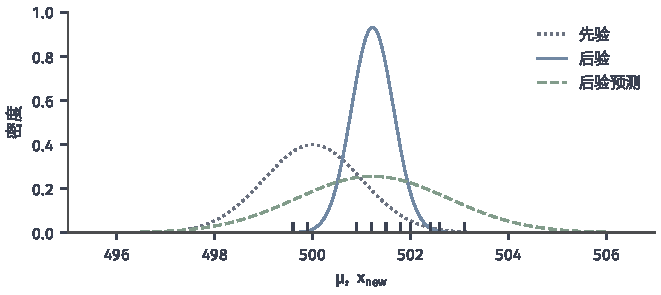
\includegraphics[width=112mm]{figures/01-basic-mathematics/05-probability-and-statistics-basics/matplotlib/pred-posterior-predictive/figure.pdf}
  \caption{灌装量的先验、后验与后验预测（$\sigma^2=2.25$已知）。灰色点线为先验$\mathcal N(500,1)$；蓝实线为观测$10$瓶后$\mu$的后验$\mathcal N(501.22,0.184)$；绿虚线为下一瓶灌装量的后验预测分布$\mathcal N(501.22,2.434)$。横轴下方的短竖线为$10$个观测值。后验描述平均灌装量的不确定性，后验预测描述单瓶灌装量的不确定性，后者宽得多。}
  \label{fig:pred-posterior-predictive}
\end{figure}

这个区间与例~\ref{ex:pred-filling-prediction}的$t$预测区间$[498.81,\,504.19]$长度相近，但依据不同：后验预测区间假定$\sigma$已知并使用了先验，概率是对给定数据下的$\mu$和$\varepsilon$计算的；$t$预测区间不需要先验，也不假定$\sigma$已知，概率是对样本和新观测的重复抽样计算的。

\section{简单线性回归中的统计推断}
\label{sec:pred-regression}

前三节的模型只有一个位置参数。许多问题关心的是两个变量之间的关系：广告投入增加时，销量平均增加多少？给定一笔预算，销量大致会是多少？本节在简单线性回归模型中回答这些问题。第~\ref{sec:ls-least-squares}节已经给出了最小二乘的计算方法，这里把它放进统计模型，依次完成估计、区间、检验与预测，并看到前三节的方法如何在同一个模型中各司其职。

全节使用下面的教学数据。

\begin{example}[广告投入与销量]
\label{ex:pred-ad-data}
某公司在$8$个城市的月广告投入$x_i$（万元）与当月销量$y_i$（百件）如下（教学数据）：
\begin{center}
\begin{tabular}{lcccccccc}
  \toprule
  城市$i$ & 1 & 2 & 3 & 4 & 5 & 6 & 7 & 8\\
  \midrule
  $x_i$ & 1 & 2 & 3 & 4 & 5 & 6 & 7 & 8\\
  $y_i$ & 3.0 & 4.4 & 4.2 & 6.0 & 5.8 & 7.6 & 6.9 & 8.9\\
  \bottomrule
\end{tabular}
\end{center}
基本汇总量为$\bar x=4.5$，$\bar y=46.8/8=5.85$，以及
\[
\begin{aligned}
 S_{xx}&=\sum_i(x_i-\bar x)^2=42,\\
 S_{xy}&=\sum_i(x_i-\bar x)(y_i-\bar y)=31.9,\\
 S_{yy}&=\sum_i(y_i-\bar y)^2=26.44.
\end{aligned}
\]
\end{example}

\subsection{线性观测模型}

\paragraph{均值响应与随机误差}

散点图（图~\ref{fig:pred-regression-bands}(a)）显示销量大致随投入线性增加，但各点并不落在一条直线上。我们把每个观测分成两部分：随投入系统变化的平均部分，以及围绕它的随机波动。

\begin{definition}[简单线性回归模型]
\label{def:pred-simple-linear-regression}
给定不全相同的实数$x_1,\dots,x_n$，设
\[
 Y_i=\beta_0+\beta_1x_i+\varepsilon_i,\qquad i=1,\dots,n,
\]
其中$\beta_0,\beta_1$是未知参数，$\varepsilon_i$是随机误差。函数$\mu(x)=\beta_0+\beta_1x$称为\term{均值响应}（mean response）。这一模型称为\term{简单线性回归}（simple linear regression），$x$称为解释变量，$Y$称为响应变量，$\beta_1$称为斜率，$\beta_0$称为截距。
\end{definition}

模型中$x_i$被当作给定的常数，只有$Y_i$是随机的。这适用于由实验者设定$x_i$的情形；若$x_i$本身也是随机观测，例如各城市的投入本身是变量，下文的结论可以理解为在观测到的$x_1,\dots,x_n$给定的条件下成立。要求$x_i$不全相同，即$S_{xx}>0$：若所有城市投入相同，数据中没有投入变化，就无法得知销量怎样随投入改变。

$\mu(x)$是响应在给定$x$处的平均值。若$\mathbb E\varepsilon_i=0$，则$\mathbb EY_i=\mu(x_i)$，由第~\ref{sec:pred-prediction}节，$\mu(x)$也就是平方误差下预测响应的最优函数。$\varepsilon_i$则包括所有未被$x$解释的因素：城市规模、季节、竞争对手等等。

\paragraph{各项假设的作用}

关于误差，我们将逐步加入四项假设。不同结论依赖不同的假设，把它们分开有助于判断某个结论在假设不成立时是否仍然可用：
\begin{center}
\begin{tabular}{p{0.3\linewidth}p{0.6\linewidth}}
  \toprule
  假设 & 支持的结论\\
  \midrule
  (A1) $\mathbb E\varepsilon_i=0$ & 均值响应确为直线；系数估计无偏\\
  (A2) $\varepsilon_i$互不相关；\newline(A3) $\operatorname{Var}\varepsilon_i=\sigma^2$都相同 & 估计量的方差公式；残差方差估计无偏\\
  (A4) $\varepsilon_i$独立且服从正态分布 & 系数估计量服从正态分布；$t$区间、检验与预测区间精确成立\\
  \bottomrule
\end{tabular}
\end{center}
(A1)是模型形式的假设：若真实关系是弯曲的，直线就系统地偏离了均值响应。(A2)与(A3)让估计量的方差有简单的形式；若误差的方差随$x$增大，后文的标准误就会失准。(A4)是精确分布理论的基础，本节的区间与检验都在(A1)--(A4)下推导，记为$\varepsilon_1,\dots,\varepsilon_n$独立同分布于$\mathcal N(0,\sigma^2)$。正态性不成立而$n$较大时，只要解释变量中没有个别取值远离其余各点，系数的区间与检验仍近似可用，因为系数估计量是许多误差的加权和，中心极限定理的想法仍然适用；但正如第~\ref{sec:pred-prediction}节所说，单个新观测的预测区间仍依赖误差的分布形状。

\subsection{回归系数的估计与残差}

\paragraph{最小二乘解}

把模型写成矩阵形式：$\bm Y=\bm X\bm\beta+\bm\varepsilon$，其中$\bm Y=(Y_1,\dots,Y_n)^\top$，$\bm\beta=(\beta_0,\beta_1)^\top$，设计矩阵$\bm X\in\mathbb R^{n\times2}$的第一列全为$1$，第二列为$(x_1,\dots,x_n)^\top$。由于$x_i$不全相同，两列线性无关，$\bm X$满列秩。按第~\ref{sec:ls-least-squares}节，使残差平方和$\lVert\bm Y-\bm X\bm\beta\rVert_2^2$最小的$\hat{\bm\beta}$由正规方程$\bm X^\top\bm X\hat{\bm\beta}=\bm X^\top\bm Y$（式~\eqref{eq:linear-algebra-normal-equations}）唯一确定。

这里的正规方程只有两个未知量，可以直接解出。写出各项，
\[
 \bm X^\top\bm X=\begin{bmatrix}n&\sum_ix_i\\\sum_ix_i&\sum_ix_i^2\end{bmatrix},\qquad
 \bm X^\top\bm Y=\begin{bmatrix}\sum_iY_i\\\sum_ix_iY_i\end{bmatrix}.
\]
第一个方程$n\hat\beta_0+\hat\beta_1\sum_ix_i=\sum_iY_i$除以$n$得$\hat\beta_0=\bar Y-\hat\beta_1\bar x$，即拟合直线经过点$(\bar x,\bar Y)$。代入第二个方程并整理，利用$\sum_ix_i^2-n\bar x^2=S_{xx}$与$\sum_ix_iY_i-n\bar x\bar Y=S_{xY}$，得到
\begin{equation}
 \hat\beta_1=\frac{S_{xY}}{S_{xx}}=\frac{\sum_i(x_i-\bar x)(Y_i-\bar Y)}{\sum_i(x_i-\bar x)^2},\qquad
 \hat\beta_0=\bar Y-\hat\beta_1\bar x.
 \label{eq:pred-ls-coefficients}
\end{equation}
称$\hat Y_i=\hat\beta_0+\hat\beta_1x_i$为\term{拟合值}（fitted value），$e_i=Y_i-\hat Y_i$为\term{残差}（residual）。正规方程等价于残差与$\bm X$的两列都正交：
\begin{equation}
 \sum_ie_i=0,\qquad\sum_ix_ie_i=0.
 \label{eq:pred-residual-orthogonality}
\end{equation}

\begin{example}[广告数据的系数估计]
\label{ex:pred-ad-fit}
由例~\ref{ex:pred-ad-data}，$\hat\beta_1=31.9/42\approx0.7595$，$\hat\beta_0=5.85-0.7595\times4.5\approx2.432$，拟合直线为$\hat y=2.432+0.7595x$。拟合值与残差（保留两位小数）为
\begin{center}
\begin{tabular}{lcccccccc}
  \toprule
  $x_i$ & 1 & 2 & 3 & 4 & 5 & 6 & 7 & 8\\
  \midrule
  $\hat y_i$ & 3.19 & 3.95 & 4.71 & 5.47 & 6.23 & 6.99 & 7.75 & 8.51\\
  $e_i$ & $-0.19$ & $0.45$ & $-0.51$ & $0.53$ & $-0.43$ & $0.61$ & $-0.85$ & $0.39$\\
  \bottomrule
\end{tabular}
\end{center}
用更多位数计算可以验证，残差之和为$0$，$\sum_ix_ie_i$也为$0$。
\end{example}

\paragraph{估计量的统计性质}

在统计模型中，$\hat\beta_0$、$\hat\beta_1$是随机变量，我们需要它们的均值与方差。注意$\sum_i(x_i-\bar x)\bar Y=0$，故$\hat\beta_1$可以写成$Y_i$的线性组合：
\[
 \hat\beta_1=\sum_ic_iY_i,\qquad c_i=\frac{x_i-\bar x}{S_{xx}}.
\]
系数满足$\sum_ic_i=0$，$\sum_ic_ix_i=\sum_i(x_i-\bar x)x_i/S_{xx}=1$，$\sum_ic_i^2=1/S_{xx}$。在(A1)下，$\mathbb E\hat\beta_1=\sum_ic_i(\beta_0+\beta_1x_i)=\beta_1$；在(A2)、(A3)下，$\operatorname{Var}(\hat\beta_1)=\sigma^2\sum_ic_i^2=\sigma^2/S_{xx}$。同理，$\bar Y=\sum_iY_i/n$与$\hat\beta_1$的协方差为$\sigma^2\sum_ic_i/n=0$，于是
\begin{equation}
 \mathbb E\hat\beta_0=\beta_0,\qquad
 \operatorname{Var}(\hat\beta_0)=\operatorname{Var}(\bar Y)+\bar x^2\operatorname{Var}(\hat\beta_1)=\sigma^2\Bigl(\frac1n+\frac{\bar x^2}{S_{xx}}\Bigr).
 \label{eq:pred-coefficient-variance}
\end{equation}
斜率的方差$\sigma^2/S_{xx}$说明：解释变量取值越分散，斜率估计越精确。这与直观一致，用两个相距很远的点确定一条直线，比用两个挨在一起的点稳定得多。在(A4)下，$\hat\beta_0$、$\hat\beta_1$是独立正态变量的线性组合，因而服从正态分布。

\paragraph{残差自由度与误差方差的估计}

$\sigma^2$未知，需要从残差估计。直接用$\frac1n\sum_ie_i^2$会偏小，因为拟合直线是从同一批数据中选出来的、尽量贴近数据的直线。偏小多少，可以从投影几何读出来。

记$\bm P=\bm X(\bm X^\top\bm X)^{-1}\bm X^\top$为到$\bm X$列空间的正交投影（式~\eqref{eq:ls-column-space-projector}），则拟合值$\hat{\bm Y}=\bm P\bm Y$，残差$\bm e=(\bm I-\bm P)\bm Y$。由于$\bm X\bm\beta$在列空间中，$(\bm I-\bm P)\bm X\bm\beta=\bm0$，所以
\[
 \bm e=(\bm I-\bm P)\bm\varepsilon.
\]
残差只含误差在列空间的正交补上的分量，见图~\ref{fig:pred-regression-projection}。列空间的维数是$2$，正交补的维数是$n-2$。

\begin{figure}[htbp]
  \centering
  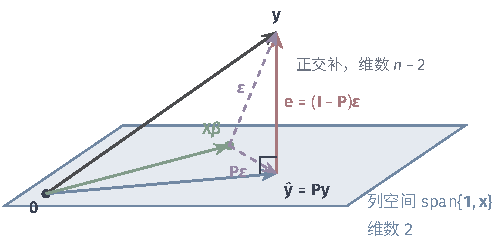
\includegraphics[width=85mm]{figures/01-basic-mathematics/05-probability-and-statistics-basics/tikz/pred-regression-projection/figure.pdf}
  \caption{简单线性回归的投影几何（示意）。$\mathbb R^n$中的平面代表设计矩阵的列空间$\operatorname{span}\{\bm 1,\bm x\}$，维数为$2$；竖直方向代表它的正交补，维数为$n-2$，图中只能画出一维。观测$\bm y=\bm X\bm\beta+\bm\varepsilon$投影为拟合值$\hat{\bm y}$；误差$\bm\varepsilon$分成列空间内的$\bm P\bm\varepsilon$（造成系数估计误差）与正交补中的$(\bm I-\bm P)\bm\varepsilon$，后者正是残差$\bm e$。}
  \label{fig:pred-regression-projection}
\end{figure}

为了计算$\mathbb E\lVert\bm e\rVert_2^2$，取正交补的一组标准正交基$\bm q_3,\dots,\bm q_n$，则$(\bm I-\bm P)\bm\varepsilon=\sum_{k=3}^n(\bm q_k^\top\bm\varepsilon)\bm q_k$，
\[
 \lVert\bm e\rVert_2^2=\sum_{k=3}^n(\bm q_k^\top\bm\varepsilon)^2.
\]
在(A2)、(A3)下，$\operatorname{Var}(\bm q_k^\top\bm\varepsilon)=\sigma^2\lVert\bm q_k\rVert_2^2=\sigma^2$，且$\mathbb E\bm q_k^\top\bm\varepsilon=0$，故$\mathbb E(\bm q_k^\top\bm\varepsilon)^2=\sigma^2$，求和得
\[
 \mathbb E\lVert\bm e\rVert_2^2=(n-2)\sigma^2.
\]
误差有$n$个分量，但其中落在列空间里的两个方向被拟合“吸收”了，留在残差中的只有$n-2$个方向。$n-2$称为残差的自由度。于是当$n>2$时，
\begin{equation}
 S^2=\frac{1}{n-2}\sum_{i=1}^ne_i^2
 \label{eq:pred-residual-variance}
\end{equation}
是$\sigma^2$的无偏估计。本节以下的$S^2$都指这个残差方差估计，它的分母是$n-2$，与单样本的修正样本方差不同。这与单样本情形的$n-1$出于同一道理：那里只拟合一个均值，列空间是$\operatorname{span}\{\bm 1\}$，失去一个自由度。

在正态假设(A4)下还能得到分布。把$\bm X$列空间的一组标准正交基$\bm q_1,\bm q_2$与$\bm q_3,\dots,\bm q_n$合起来，得到正交矩阵$\bm Q$。由第~\ref{sec:rvec-gaussian}节，$\bm\varepsilon\sim\mathcal N(\bm 0,\sigma^2\bm I)$经正交变换后$\bm Q^\top\bm\varepsilon\sim\mathcal N(\bm 0,\sigma^2\bm I)$，即$\bm q_1^\top\bm\varepsilon,\dots,\bm q_n^\top\bm\varepsilon$独立同分布于$\mathcal N(0,\sigma^2)$。因此：
\begin{itemize}
  \item $\lVert\bm e\rVert_2^2/\sigma^2=\sum_{k=3}^n(\bm q_k^\top\bm\varepsilon/\sigma)^2\sim\chi^2_{n-2}$，即$(n-2)S^2/\sigma^2\sim\chi^2_{n-2}$；
  \item $\hat{\bm\beta}=(\bm X^\top\bm X)^{-1}\bm X^\top\bm P\bm Y$只依赖$\bm P\bm Y=\bm X\bm\beta+\sum_{k=1}^2(\bm q_k^\top\bm\varepsilon)\bm q_k$，而$S^2$只依赖$\bm q_3^\top\bm\varepsilon,\dots,\bm q_n^\top\bm\varepsilon$，所以$\hat{\bm\beta}$与$S^2$独立。
\end{itemize}
这正是第~\ref{sec:samp-normal}节用正交旋转证明样本均值与样本方差独立、$(n-1)S^2/\sigma^2\sim\chi^2_{n-1}$的同一论证：单样本时列空间是$\operatorname{span}\{\bm 1\}$，只有一维；这里换成了二维。

\begin{example}[广告数据的残差方差]
\label{ex:pred-ad-residual-variance}
由例~\ref{ex:pred-ad-fit}的残差，$\sum_ie_i^2\approx2.211$，自由度$n-2=6$，$s^2\approx2.211/6\approx0.3685$，$s\approx0.607$。作为对照，$S_{yy}=26.44$是不使用$x$、只用$\bar y$拟合时的残差平方和；引入广告投入后残差平方和降到其$8.4\%$，即投入的线性变化解释了销量总波动的约$91.6\%$。
\end{example}

\subsection{回归系数的区间估计与检验}

\paragraph{标准误、$t$区间与检验}

把$\operatorname{Var}(\hat\beta_1)=\sigma^2/S_{xx}$中的$\sigma$换成$S$，得到斜率的估计标准误$\operatorname{se}(\hat\beta_1)=S/\sqrt{S_{xx}}$。在(A1)--(A4)下，$(\hat\beta_1-\beta_1)/(\sigma/\sqrt{S_{xx}})\sim\mathcal N(0,1)$，$(n-2)S^2/\sigma^2\sim\chi^2_{n-2}$，二者独立，按$t$分布的定义，
\begin{equation}
 \frac{\hat\beta_1-\beta_1}{S/\sqrt{S_{xx}}}\sim t_{n-2}.
 \label{eq:pred-slope-t}
\end{equation}
这是与单样本$t$统计量~\eqref{eq:pred-t-pivot}完全平行的枢轴量，只是自由度变为$n-2$。由此得到斜率的置信区间$\hat\beta_1\pm t_{n-2,1-\alpha/2}\,S/\sqrt{S_{xx}}$，以及$H_0:\beta_1=b$的$t$检验。最常见的是$H_0:\beta_1=0$，即均值响应不随$x$变化。截距同理，标准误为$S\sqrt{1/n+\bar x^2/S_{xx}}$。

\begin{example}[广告数据的斜率推断]
\label{ex:pred-ad-slope}
$\operatorname{se}(\hat\beta_1)=0.607/\sqrt{42}\approx0.0937$，$t_{6,0.975}\approx2.447$，斜率的$95\%$置信区间为
\[
 0.7595\pm2.447\times0.0937=[0.530,\,0.989].
\]
检验$H_0:\beta_1=0$，$t=0.7595/0.0937\approx8.11$，自由度$6$，双侧$p\approx0.0002$，拒绝$H_0$。截距的标准误为$0.607\times\sqrt{1/8+4.5^2/42}\approx0.473$，$95\%$区间为$2.432\pm2.447\times0.473\approx[1.27,\,3.59]$。截距是$x=0$即完全不投放广告时的平均销量，但数据中最小的投入是$1$万元，这个区间依赖直线在$[0,1]$上仍然成立，应当谨慎解读。
\end{example}

\paragraph{关联、效应大小与因果}

$H_0:\beta_1=0$被拒绝，说明在模型假设下，销量的均值与广告投入有线性关联。它没有说明关联有多强，这要看估计值和区间：投入每增加$1$万元，平均销量估计增加约$76$件，$95\%$置信区间约为$53$到$99$件。这才是实际决策需要的效应大小。

更重要的是，回归系数描述的是“投入较高的城市，销量平均较高”，而不是“提高投入会使销量增加”。在这批观测数据中，投入并不是随机分配的：公司很可能向市场规模大的城市投入更多，而市场规模本身就会带来更高的销量。这时$\hat\beta_1$混合了广告的作用与城市规模的作用，无论$p$值多小都无法将二者分开。若由研究者随机决定各城市的投入，城市规模等因素就与投入无关，斜率才可以解释为投入的平均因果作用。统计显著性只回答“关联是否可能由随机波动造成”，不回答“关联从何而来”。因果作用的定义与识别条件见\BookChapterRef{chap:causal-inference}{卷4《数学准备：流形、概率分布与统计推断》的“因果响应”章}。

\subsection{均值响应与新观测的预测}

\paragraph{均值响应的置信区间}

给定投入$x_0$，城市的平均销量是$\mu(x_0)=\beta_0+\beta_1x_0$，其估计为$\hat\mu(x_0)=\hat\beta_0+\hat\beta_1x_0$。利用$\hat\beta_0=\bar Y-\hat\beta_1\bar x$改写为
\[
 \hat\mu(x_0)=\bar Y+\hat\beta_1(x_0-\bar x).
\]
上面已经算出$\bar Y$与$\hat\beta_1$不相关，方差直接相加：
\begin{equation}
 \operatorname{Var}\bigl(\hat\mu(x_0)\bigr)=\frac{\sigma^2}n+(x_0-\bar x)^2\frac{\sigma^2}{S_{xx}}
 =\sigma^2\Bigl(\frac1n+\frac{(x_0-\bar x)^2}{S_{xx}}\Bigr).
 \label{eq:pred-mean-response-variance}
\end{equation}
第一项是整条直线上下平移的不确定性，第二项是斜率的不确定性在$x_0$处造成的波动，它随$x_0$与$\bar x$的距离平方增长。拟合直线像一根绕着$(\bar x,\bar Y)$转动的杆，离支点越远，摆动越大。

$\hat\mu(x_0)$是$\hat{\bm\beta}$的线性函数，在(A4)下服从正态分布并与$S^2$独立，因此
\[
 \hat\mu(x_0)\pm t_{n-2,1-\alpha/2}\,S\sqrt{\frac1n+\frac{(x_0-\bar x)^2}{S_{xx}}}
\]
是$\mu(x_0)$的置信水平为$1-\alpha$的置信区间。

\paragraph{新观测的预测区间}

若要预测投入为$x_0$的某个城市的实际销量$Y_0=\mu(x_0)+\varepsilon_0$，其中$\varepsilon_0\sim\mathcal N(0,\sigma^2)$与已有数据独立，则与第~\ref{sec:pred-prediction}节一样，预测误差$Y_0-\hat\mu(x_0)$包括新观测的噪声和估计误差两部分，方差相加：
\[
 \operatorname{Var}\bigl(Y_0-\hat\mu(x_0)\bigr)=\sigma^2\Bigl(1+\frac1n+\frac{(x_0-\bar x)^2}{S_{xx}}\Bigr).
\]
按同样的论证得到$Y_0$的预测区间
\begin{equation}
 \hat\mu(x_0)\pm t_{n-2,1-\alpha/2}\,S\sqrt{1+\frac1n+\frac{(x_0-\bar x)^2}{S_{xx}}}.
 \label{eq:pred-regression-prediction-interval}
\end{equation}
与均值区间相比，根号中多出的$1$对应新观测的噪声，不随样本量增大而消失。$x_0=\bar x$时，两种区间分别回到第~\ref{sec:pred-intervals}节的均值区间与第~\ref{sec:pred-prediction}节的预测区间的形式，只是自由度为$n-2$。

\begin{example}[投入$6$万元时的两种区间]
\label{ex:pred-ad-intervals}
取$x_0=6$，$\hat\mu(6)=2.432+0.7595\times6\approx6.989$，$(x_0-\bar x)^2/S_{xx}=2.25/42\approx0.0536$。
\begin{itemize}
  \item 均值响应：标准误$0.607\sqrt{0.125+0.0536}\approx0.257$，$95\%$置信区间$6.989\pm2.447\times0.257\approx[6.36,\,7.62]$；
  \item 新观测：标准误$0.607\sqrt{1+0.125+0.0536}\approx0.659$，$95\%$预测区间$6.989\pm2.447\times0.659\approx[5.38,\,8.60]$。
\end{itemize}
前者说投入$6$万元的城市平均销量在$636$到$762$件之间；后者给出某个投入$6$万元的城市的销量范围：$538$到$860$件，按$95\%$的预测水平构造。预测区间约为均值区间的$2.6$倍宽。
\end{example}

图~\ref{fig:pred-regression-bands}(a)把所有$x_0$处的两种区间连成两条带。均值置信带在$\bar x=4.5$处最窄，向两侧张开；预测带宽得多，且由于根号中的$1$占主导，看起来几乎是平行的。

\begin{figure*}[htbp]
  \centering
  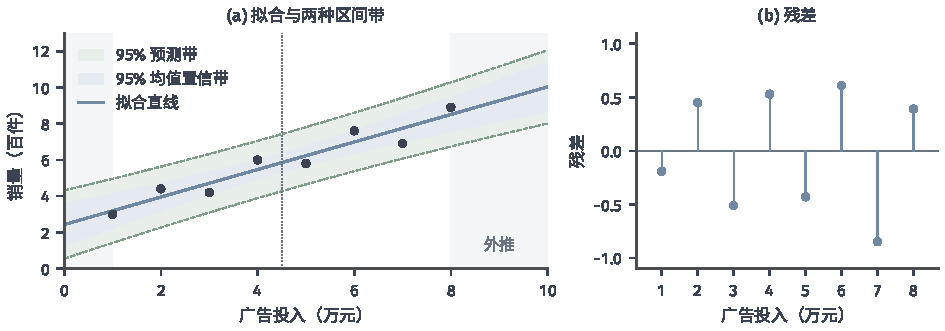
\includegraphics[width=160mm]{figures/01-basic-mathematics/05-probability-and-statistics-basics/matplotlib/pred-regression-bands/figure.pdf}
  \caption{广告数据的简单线性回归。(a) 黑点为$8$个城市的观测，蓝线为拟合直线$\hat y=2.432+0.7595x$；蓝色窄带为均值响应的$95\%$置信带，绿色宽带（虚线为边界）为新观测的$95\%$预测带，二者都由$t_{6,0.975}$与$s\approx0.607$计算。点线标出$\bar x=4.5$，置信带在此处最窄。灰色区域$x<1$与$x>8$超出了观测范围，那里的带只在直线关系继续成立时才有意义。(b) 各城市的残差，没有明显的弯曲趋势或随$x$扩大的波动。}
  \label{fig:pred-regression-bands}
\end{figure*}

\paragraph{残差检查与外推}

以上所有区间都以(A1)--(A4)为前提，而这些假设可以部分地用残差来检查。若真实关系是弯曲的，残差会随$x$呈现系统的弧形；若误差方差随$x$增大，残差的散布会呈喇叭形；个别远离其余点的残差提示异常观测。图~\ref{fig:pred-regression-bands}(b)中残差正负交替，大小没有随$x$明显变化，看不出违背假设的迹象。只有$8$个观测时，这种检查的能力很有限，只能发现明显的问题。

外推需要格外小心。取$x_0=10$，公式给出均值响应的$95\%$区间约$[8.66,\,11.39]$，预测区间约$[8.01,\,12.05]$，都比$x_0=6$时宽，这反映了式~\eqref{eq:pred-mean-response-variance}中距离项的增长。但这种加宽只计入了模型成立时的估计误差，没有计入模型本身出错的可能：数据只覆盖$1$到$8$万元，投入继续增加时，销量很可能因市场饱和而增长放缓。在观测范围之外，直线是否仍然成立，数据本身无法回答，区间公式也无从反映。

\section{本章小结}
\label{sec:pred-summary}

本章回答了章首的三个问题。对平均灌装量，我们构造了置信区间$[500.69,\,502.31]$；对“平均灌装量等于$500$”，$t$检验给出$p\approx0.002$；对下一瓶，预测区间为$[498.81,\,504.19]$。三个结果使用同一批数据和同一个抽样分布理论，却回答不同的问题。表~\ref{tab:pred-summary}按目标对象、所用随机性、构造依据和概率含义把它们并列比较。

\begin{table*}[htbp]
  \centering
  \begin{tabularx}{\linewidth}{@{}p{0.12\linewidth}XXXX@{}}
    \toprule
    方法 & 目标对象 & 随机性来源 & 构造依据 & 概率含义\\
    \midrule
    置信区间 & 固定的未知参数 & 样本在重复抽样中的变化 & 枢轴量的抽样分布 & 规则以$1-\alpha$的概率覆盖真参数\\
    可信区间 & 参数 & 给定数据时参数的后验分布 & 先验与似然得到的后验 & 参数落在区间中的后验概率为$1-\alpha$\\
    假设检验 & 关于参数的陈述 & 原假设下样本的变化 & 原假设下统计量的分布 & $H_0$为真时错误拒绝的概率不超过$\alpha$\\
    预测区间 & 未来的单个观测 & 样本与新观测的联合变化 & 新观测与估计量之差的分布 & 区间以$1-\alpha$的概率覆盖新观测\\
    \bottomrule
  \end{tabularx}
  \caption{本章四类推断方法的比较。前三类的对象都是参数，预测区间的对象是随机变量；可信区间的概率对参数计算，其余三类的概率对样本计算。}
  \label{tab:pred-summary}
\end{table*}

区间估计的共同方法是从枢轴量反解参数。正态模型下的均值$t$区间与方差卡方区间是精确的；均值区间在一般总体下还有中心极限定理提供的渐近保证，方差区间则完全依赖正态性。比例的区间面临离散性：Wald区间在小样本与边界附近覆盖不足，Clopper--Pearson区间以保守为代价保证覆盖。可信区间给出关于参数的直接概率陈述，但它的频率覆盖率取决于先验是否恰当。

假设检验先在原假设下控制第一类错误，再由效应大小、噪声与样本量决定功效。$p$值报告证据的强度，但它既不是原假设为真的概率，也不衡量效应的大小；不拒绝原假设也不证明它成立。同一族检验与同一族置信区间互为反演，只有构造规则匹配时，才能用区间直接判断检验。配对与独立设计、等方差与否、精确与近似计算，都会改变检验的结论。

预测的对象是随机变量，误差由新观测的噪声和参数估计误差两部分组成。增加样本只能减少后者，所以预测区间的半宽因子$\sqrt{1+1/n}$始终不小于$1$，而均值区间的$1/\sqrt n$趋于零。后验预测分布把这两部分写成一个积分，同样包含观测噪声与参数后验方差。

简单线性回归把以上任务放进一个模型：最小二乘给出系数，投影几何说明残差有$n-2$个自由度并给出$\sigma^2$的无偏估计，斜率的$t$区间与检验刻画线性关联，均值响应区间与预测区间分别回答“平均是多少”和“下一个是多少”。回归的显著性不等于因果，区间公式也不覆盖观测范围以外的模型误差。这些结论依赖的假设，需要用残差与研究设计来检验。
